\startdocument

\section{String Inflation}
\label{sec:Sinfla}

\subsection{Embedding Inflation in String Theory}

As described in Section \ref{SecCO}, inflation is the leading candidate theory for the origin of structure in the universe. This reason alone would justify attempts to embed inflation in string theory (see \cite{Quevedo:2002xw,Kallosh:2007ig,Burgess:2004jk,Burgess:2006nod,Burgess:2006uv,Cline:2006hu,HenryTye:2006uv,McAllister:2007bg,Copeland:2011dx,Cicoli:2011zz,Burgess:2011fa, Yamaguchi:2011kg, Burgess:2013sla,Baumann:2014nda,Silverstein:2016ggb,Nastase:2019mhe} for detailed reviews on different aspects of string cosmology and inflation in string theory). However, there are more specific reasons why a consistent theory of quantum gravity is necessary for a full understanding of the inflationary dynamics.

\subsubsection{Motivations for String Inflation}

There are several reasons to require a consistent embedding of inflation models within 
string theory. Below, we list those which we consider most relevant: 

\begin{itemize}

\item \emph{UV sensitivity of inflation}: As we discussed in Section \ref{sec:infla}, single-field inflation is driven by the dynamics of a scalar field with mass $M_{\rm inf}$ below the Hubble scale during inflation $H_{\rm inf}$. This can be see from the  second potential slow-roll parameter $\eta_V$ introduced in \eqref{eq:etaV}, which  can be expressed as
\begin{equation}
\setlength\fboxsep{0.25cm}
\setlength\fboxrule{0.4pt}
\boxed{
\eta_V\simeq \left|\frac{M_{\rm inf}^2}{H^2}\right|\ll 1\,,
\label{etaProb}
}
\end{equation}
where the condition $\eta_V \ll 1$ guarantees that inflation lasts for long enough to solve the horizon problem and flatness problems. However, in the absence of a protection mechanism based on (approximate) symmetries, quantum corrections are expected to make these scalars heavy, so that $\eta_V\simeq \mathcal{O}(1)$. 

There are two generic sources of $\mathcal{O}(1)$ corrections to the $\eta_V$-parameter. First, quantum effects tend to generate corrections to scalar masses of order the cut-off of the effective field theory $\Lambda$, $M_{\rm inf}\simeq \mathcal{O}(\Lambda)$. For controlled inflationary model building with $H_{\rm inf}\lesssim \Lambda$, one has from (\ref{etaProb}) $\eta_V \gtrsim 1$. Secondly, even if the scalar potential arising from relevant and marginal operators yields $\eta_V \ll 1$, irrelevant operators of the form
\begin{equation}
\setlength\fboxsep{0.25cm}
\setlength\fboxrule{0.4pt}
\boxed{
    \Delta V = c\, V(\phi)\left(\frac{\phi}{\Lambda}\right)^2\,,
}
\end{equation}
would produce a correction to $\eta_V$ of order 
\begin{equation}
\setlength\fboxsep{0.25cm}
\setlength\fboxrule{0.4pt}
\boxed{
    \Delta \eta_V = 2 c \left(\frac{M_{\rm Pl}}{\Lambda}\right)^2\quad\text{with}\quad \Lambda \lesssim M_{\rm Pl}\,,
}
\end{equation}
that would violate the slow-roll condition if $\Lambda \ll M_{\rm Pl}$, or if $c\simeq \mathcal{O}(1)$ for $\Lambda \simeq M_{\rm Pl}$. 

This is usually referred to as the $\eta_V$-problem in  single-field inflation. A solution to it, if not based on fine-tuning, requires the presence of symmetries which can be only  provided by a consistent UV embedding. These symmetries, even if not exact (as for the case of global symmetries in quantum gravity),  may be enough to explain why $c \ll 1$. This UV-sensitivity of inflation implies that inflationary model building 
can only be trusted with a knowledge of its UV completion. Note that a robust UV embedding is needed even if the $\eta_V$-problem is addressed by relying on fine-tuning, since one has to ensure that the underlying theory features enough freedom to allow $\eta_V$ to be 
tuned to a small value.

On the other hand, as we discussed in Section \ref{sec:multinf}  the $\eta_V$ parameter in multi-field inflation, \eqref{etaVmulti}, does not have to be small. Indeed, the masses of the inflatons can be larger than the Hubble scale $H_{\rm inf}$ during inflation without affecting slow-roll \cite{Chakraborty:2019dfh,Aragam:2021scu}\footnote{We discuss an example of this below. See Appendix A of \cite{Chakraborty:2019dfh} for  a list of examples in field theory, and \cite{Aragam:2021scu} for  more details and examples in supergravity.}. The problem of UV sensitivity of inflation in this case cannot be formulated in terms of the inflaton masses, i.e.~$\eta_V^m$ of Eq.~\eqref{etaVmulti}. 

\item \emph{Trans-Planckian field excursions and the tensor-to-scalar ratio}: We saw in Eq. (\ref{LythBound}), reproduced here, that the size of the tensor fluctuation can be related to the field displacement of the inflaton by,

\be
\setlength\fboxsep{0.25cm}
\setlength\fboxrule{0.4pt}
\boxed{
 \frac{\Delta\varphi}{\Mp} = \int^{N_{\rm hc}}_{N_{\rm end}}{ dN \,\sqrt{\frac{r}{8}} } \,.
 \label{Lyth2}
 }
 \ee
Large and observable values of the tensor-to-scalar ratio $r$ correspond to trans-Planckian field excursions of the inflaton $\varphi$. Indeed, the simplest field theory models of single-field  inflation, such as chaotic inflation, all lead to substantially trans-Planckian field excursions (see Eqs.~\eqref{eq:monoinf}-\eqref{eq:natuinf} in Sec.~\ref{sec:infla}).

Eq.~(\ref{Lyth2}) represents a rare example where the Planck scale -- the quantum gravity energy scale -- explicitly appears inside a quantity that is observable, not only in principle but also possibly in practice with current technology. By definition, a trans-Planckian inflationary field excursion requires the existence of a potential within the UV-complete theory that sustains an approximately de Sitter phase across a Planckian distance in field space. Whether such regions can exist can only be answered within a quantum gravity theory.  For any potential $V_{inf} (\varphi)$, generic non-renormalisable corrections with $\mc{O}(1)$ coefficients $\lambda_n$,
\be
\setlength\fboxsep{0.25cm}
\setlength\fboxrule{0.4pt}
\boxed{
V_{full}(\varphi) = V_{inf}(\varphi) + \sum \lambda_n \frac{\varphi^n}{\Mp^n},
\label{ghjt}
}
\ee
will destroy the flatness of trans-Planckian field excursions. Whereas the $\eta_V$ problem only required control over the quadratic term in the potential, flatness on trans-Planckian scales requires control over all terms in Eq. (\ref{ghjt}).  

Again, the multi-field case is more subtle. In that case, $\Delta\varphi$ corresponds to the multi-field {\em inflationary trajectory}. This may or  not, coincide with the {\em geodesic trajectory} in field space, which in general will be curved. 
Thus in the multi-field case, the potential can be very steep (indicating the possibility of heavy inflatons, as discussed before), while inflation proceeds along a suitable flat non-geodesic trajectory, i.e.~$\Omega/H\gtrsim 1$, along which $\epsilon_V^m, \eta_V^m\gtrsim 1$ (see Eqs.~\eqref{eq:w}, \eqref{epsimulti}, \eqref{etaVmulti})\footnote{Moreover, when more than one scalar field is active during inflation, entropic perturbations may be converted -- more or less effectively -- into adiabatic perturbations, introducing a  {\em transfer angle} $\Theta$ \cite{Wands:2002bn} in \eqref{Lyth2} through $r=16\,\epsilon\cos^2\Theta$.}.
 
Having a UV-complete theory of quantum gravity, such as string theory, thus allows to address 
questions about the structure of the potential and whether it supports geodesic (single-field) or non-geodesic  trans-Planckian field excursions. 
This is especially relevant given 
that many of the best known field theory models of inflation, such as chaotic inflation or natural inflation, require trans-Planckian field excursions. The difficulties of attaining flat potentials over such field excursions in string theory has been appreciated for a long time (e.g. see \cite{Banks:2003sx}) and has recently received renewed attention with the Swampland Distance Conjecture (see the discussion in section \ref{sec:Alt}).

\item \emph{UV constraints on model building}: Field theoretic models of inflation can be characterised by almost any kind of inflationary potential, with very different predictions for the main cosmological observables. However the requirement of a sensible embedding into string theory, based on explicit Calabi-Yau realisations with full moduli stabilisation, can strongly constrain the allowed shape of the inflationary potential.

\item \emph{Connection to observations}: Inflation represents a unique possibility to test high scale physics like string theory due to the fact that the inflation scale is expected to be not too far from the Planck scale. Moreover, string theory applications to inflation may lead to the discovery of features which are either generic in the string landscape, or alternatively impossible to achieve from string theory with control over the effective field theory (one case may be large primordial tensor modes together with low-energy supersymmetry). 
Such predictions can lead to sharper tests of string theory scenarios, in particular through studying the interplay between cosmology and particle physics within the same model. 

\item \emph{Initial conditions}: Embedding inflation into string theory can help to understand the delicate issue of initial conditions and the mechanism through which inflation started.

\item \emph{Reheating}: A complete understanding of reheating after the end of inflation requires the knowledge of all relevant degrees of freedom at inflationary energies to make sure that the inflaton energy density is transferred to the production of Standard Model degrees of freedom without too much energy being lost into hidden sector particles. To perform this analysis it is clearly crucial to have a robust UV embedding of inflation into string theory to control all the microscopic degrees of freedom.
\end{itemize}

\subsubsection{Requirements for String Inflation}

Besides the reasons to embed inflation into string theory, let us briefly discuss what are the main conditions that a perfect working model of string inflation should satisfy: 

\begin{itemize}
\item \emph{Moduli stabilisation}: All the closed and open string moduli should be stabilised. The scalar potential should feature a region suitable to drive inflation without any orthogonal runaway direction which would destabilise the inflationary dynamics. Ideally, the same scalar potential should also allow for a proper description of the late-time evolution of the universe, including both the reheating epoch and also either a de Sitter minimum or a quintessence direction. 

\item \emph{Hierarchies:} A controlled low-energy effective field theory should be characterised by the following mass hierarchy throughout the whole inflationary dynamics:
\bea
&&\label{eq:standardH}
M_{\rm inf}< H_{\rm inf} < M_{\rm KK} < M_s < M_{\rm Pl}\,, \qquad {\text{ standard hierarchy, single and multi-field}}\\
&&
H_{\rm inf} < M_{\rm inf}<M_{\rm KK} < M_s < M_{\rm Pl}\,, \qquad {\text{ multi-field inflation }}
\label{eq:multiH}
\eea
where $H_{\rm inf}$ is the Hubble scale during inflation and $M_{\rm inf}$ denotes the inflaton mass during inflation. In the multi-field case, it denotes the eigenvalues of the mass matrix ${\mathbb M}^a_{\,\,\,b}=\nabla^a\nabla_b V$ along the inflationary trajectory.  
In the standard hierarchy case \eqref{eq:standardH},   all the moduli with mass $m\gtrsim H_{\rm inf}$ are heavy and sit at their minimum during inflation. The moduli with a mass of order the Hubble scale during inflation or smaller, $m\lesssim H_{\rm inf}$, should be analysed in detail as they can affect the inflationary dynamics. In this sense, the cleanest situation is the single-field case where all the moduli different from the inflaton can be decoupled since they are heavier than the Hubble scale. Other scenarios are instead intrinsically multi-field and need a deeper analysis (one possible exception involves additional axion fields which always remain massless and decouple from the dynamics). Let us also stress that the requirement to realise inflation below the Kaluza-Klein and the string scale is just due to our poor understanding of the full dynamics involving stringy corrections but it does not need to be a regime preferred by Nature.

\item \emph{Computational control}: Any scalar potential receives quantum corrections of several kinds in different regions of the underlying parameter and field spaces. Hence any working model of accelerated expansion needs to have computational control over the effective field theory. This requires that the size of all cycles should be fixed above the string scale and both the $\alpha'$ and the string loop perturbative expansions should be under control. Leading and higher order non-perturbative effects should also be computable and the backreaction from fluxes and localised objects should also be suppressed, or properly included.

\item \emph{Calabi-Yau embedding}: In order to have a successful model of inflation from string theory, a string-inspired supergravity setup is clearly not enough. Ideally, one should build a globally consistent Calabi-Yau (or equivalent) compactification with a rigorous description of the underlying geometry and topology, and an explicit orientifold involution and brane setup. In this way one can have control over the underlying K\"ahler cone which determines the field space, and can check if the brane setup and the divisors have the right topology to generate the desired perturbative corrections to the K\"ahler potential and instanton contributions to the superpotential to freeze the moduli and generate the inflationary potential. Given that the real world does not feature just an initial epoch of accelerated expansion, the same Calabi-Yau compactification should allow for the realisation of a Standard Model-like sector with a non-Abelian gauge group and chiral matter, together with a viable reheating process to produce it after the end of inflation. 

\item \emph{Comparison with data}: An ideal working model of string inflation should clearly match all existing data about cosmological observables. The main data to fit are the scalar spectral index and the amplitude of the density perturbations, together with the present upper bound on tensor modes. Stringent bounds arise also from non-Gaussianities and the amplitude of isocurvature modes which become particularly relevant in multi-field models. In fact, fields which are lighter than the inflaton, like ultra-light axions typical of string compactifications, might behave during inflation just as spectator fields which acquire isocurvature fluctuations that might be in tension with data if their later contribution to dark matter is considerable. Moreover bounds from dark radiation and dark matter overproduction should be respected in the reheating and post-inflationary epoch. 

\item \emph{Novel predictions}: Ideally, a successful model will also produce novel predictions for upcoming experiments that are characteristic of the scenario and also distinguish it from other related models.

\end{itemize}

It is clear that no existing model in the literature satisfies all these requirements perfectly. However, it is useful to hold them all in mind as the ultimate aspirational target.

\subsection{Single-Field Inflation}

Let us start our discussion with the case where only one modulus remains light and can be identified with the inflaton, or where more fields are light but the cosmological predictions remain effectively those of single-field inflation. The most robust models are based on shift symmetries which protect the flatness of the inflationary potential and provide an elegant solution to the $\eta_V$-problem in single-field inflation. These shift symmetries are always approximate and can be either saxionic, in the case of K\"ahler moduli \cite{Burgess:2014tja,Burgess:2016owb}, or axionic, in the case of $C_0$, $C_2$, $C_4$ and complex structure axions \cite{Pajer:2013fsa}. Denoting schematically the relevant complex modulus as $T = \tau + {\rm i} \theta$, saxionic shift symmetries look like:
\begin{equation}
T \to T' = T + \alpha\, , \quad \alpha \in \mathbb{R}\qquad \Rightarrow \qquad \tau \to \tau' = \tau + \alpha\,,
\label{rhoshift}
\end{equation}
while axionic shifts take the form:
\begin{equation}
T \to T' = T+ {\rm i} \alpha\, , \quad\alpha \in \mathbb{R} \qquad \Rightarrow \qquad \theta \to \theta' = \theta + \alpha\,.
\label{axionshift}
\end{equation}
Depending on the effects which break these symmetries, the inflationary potential can take different forms. 

In the absence of a symmetry-based mechanism to solve the single-field $\eta_V$-problem, accelerated expansion can still be achieved through an appropriate fine-tuning of the underlying parameters which allows for cancellations among higher dimensional operators that would otherwise ruin the solution. Let us now present a broad overview of different single-field models of string inflation classifying them in terms of the mechanism exploited to realise inflation: based on either saxionic/axionic shift symmetries or fine-tuning.





\subsubsection{Exponential Potentials from Saxionic Shift Symmetries}

Due to the typical no-scale structure of type IIB flux compactifications (a structure to the effective field theory which is special and absent in `generic' theories) \cite{Cremmer:1983bf,Burgess:2020qsc}, which holds at tree-level and even at 1-loop order in type IIB, the K\"ahler moduli different from the overall volume mode enjoy an effective non-compact shift symmetry of the type (\ref{rhoshift}). In fact, all the K\"ahler moduli are flat at tree-level. Due to the extended no-scale structure which suppresses the contributions of string loops \cite{Cicoli:2007xp}, the first effect which generates a potential is at $\mathcal{O}(\alpha'^3)$ \cite{Becker:2002nn}. However, this higher derivative effect depends just on the overall volume $\mathcal{V}$, leaving all the other moduli flat at this order of approximation. Hence, all the K\"ahler moduli orthogonal to the volume mode are in principle promising inflaton candidates since they are leading order flat directions. 

Different effects can break their shift symmetry and generate the inflationary potential. These can be $\mathcal{O}(\alpha'^3)$ corrections at $(F$-${\rm term})^4$ level \cite{Ciupke:2015msa}, $\mathcal{O}(\alpha'^4 g_s^2)$ string loop effects \cite{Berg:2005ja,vonGersdorff:2005bf,Berg:2007wt,Cicoli:2008va}, or even non-perturbative corrections. In the end, their effect can be captured by exponential contributions of the form $V_0\,e^{\pm \phi/f}$, where $f$ is an effective decay constant whose value depends on the topology of the K\"ahler modulus and the nature of the symmetry breaking effect. Generically, $g_s$ and $\alpha'$ perturbative corrections are power-law in terms of the canonically unnormalised moduli $\tau$ \cite{Cicoli:2021rub}, and become exponential in terms of the canonically normalised field $\phi$ since $\tau = e^{\phi/f}$. On the other hand, non-perturbative corrections are exponential in terms of the original moduli $\tau$, and remain exponential after canonical normalisation since they are relevant just for blow-up and Wilson moduli whose canonical normalisation is power-law. Therefore, the resulting inflationary potential for the canonically normalised field $\phi$ in the plateau region which sustains inflation takes the schematic form (we ignore additional contributions which guarantee the presence of a minimum after the end of inflation):
\begin{equation}
\setlength\fboxsep{0.25cm}
\setlength\fboxrule{0.4pt}
\boxed{
V = V_0 \left(1-{\cal C}_0\,e^{-(\phi/f)^p}\right),
}
\label{Refeq}
\end{equation}
where ${\cal C}_0$ is a constant depending on the details of the model. 
Different K\"ahler moduli correspond to different values of the effective decay constant $f$. We list the main models proposed in the literature:

\subsubsection*{Fibre Inflation}

In this case the inflaton is the volume of a K3 or $T^4$ divisor and the Calabi-Yau is a fibration over a $\mathbb{P}^1$ base \cite{Cicoli:2011it}. The potential can be generated by various perturbative corrections: $\mathcal{O}(g_s^2 \alpha'^4)$ and $\mathcal{O}(g_s^4 \alpha'^4)$ string loops \cite{Cicoli:2008gp}; $\mathcal{O}(g_s^4 \alpha'^4)$ string loops and $\mathcal{O}(\alpha'^3)$ effects at $(F$-${\rm term})^4$ level \cite{Broy:2015zba}; $\mathcal{O}(g_s^2 \alpha'^4)$ string loops and $\mathcal{O}(\alpha'^3)$ corrections at $(F$-${\rm term})^4$ order \cite{Cicoli:2016chb}. 

In each case the effective decay constant is $\mathcal{O}(1)$ in Planck units. More precisely, the original model features a potential that in the inflationary region matches (\ref{Refeq}) with $f=M_{\rm Pl}/\sqrt{3}$, $p=1$ and ${\cal C}_0=4$. The total inflationary potential is of the form (setting $\Mp=1$):
\begin{equation}
\setlength\fboxsep{0.25cm}
\setlength\fboxrule{0.4pt}
\boxed{
V =V_0\left[3-4\,e^{-\frac{1}{\sqrt{3}}\phi} + e^{-\frac{4}{\sqrt{3}}\phi} + \delta \left(e^{\frac{2}{\sqrt{3}}\phi}-1\right)\right],
}
\end{equation}
where $\delta \propto g_s^4 \ll 1$. See Fig. \ref{Fig:Fiber} for a qualitative plot of this potential. This model is characterised by a trans-Planckian inflaton field range of order $\Delta\phi\simeq \mathcal{O}(5)\,M_{\rm Pl}$ \cite{Cicoli:2018tcq} which corresponds to $H_{\text{inf}}\simeq 5\times 10^{13}$ GeV. Ref. \cite{Cicoli:2020bao} performed a detailed analysis determining the values of the microscopic parameters which give the best fit to the most recent cosmological datasets, obtaining $n_s = 0.9696^{+0.0010}_{-0.0026}$ and $r = 0.00731^{+0.00026}_{-0.00072}$ at $68\%$ CL (for Planck 2018 temperature and polarisation data only) at $N_e\simeq 52$ efoldings (see \cite{Bhattacharya:2020gnk} for an analysis making making use of cobaya \cite{Torrado:2020dgo}
and modechord \cite{Handley:2015fda}). 

This construction is among the best developed string inflationary models since it features: moduli stabilisation, globally consistent Calabi-Yau embeddings with chiral matter on D7-branes \cite{Cicoli:2016xae,Cicoli:2017axo}, analysis of preheating effects \cite{Antusch:2017flz,Gu:2018akj}, study of perturbative reheating for Standard Model sectors 
on both D3-branes \cite{Cicoli:2022uqa} and D7-branes \cite{Cicoli:2018cgu}, analysis of the production of primordial black holes \cite{Cicoli:2018asa} and the associated generation of secondary gravity waves \cite{Cicoli:2022sih}, study of the behaviour of axionic isocurvature modes \cite{Cicoli:2018ccr,Cicoli:2019ulk,Cicoli:2021yhb,Cicoli:2021itv}, production of a CMB power loss at large angular scales \cite{Cicoli:2013oba, Cicoli:2014bja}.

\begin{figure}[t]
\begin{center}
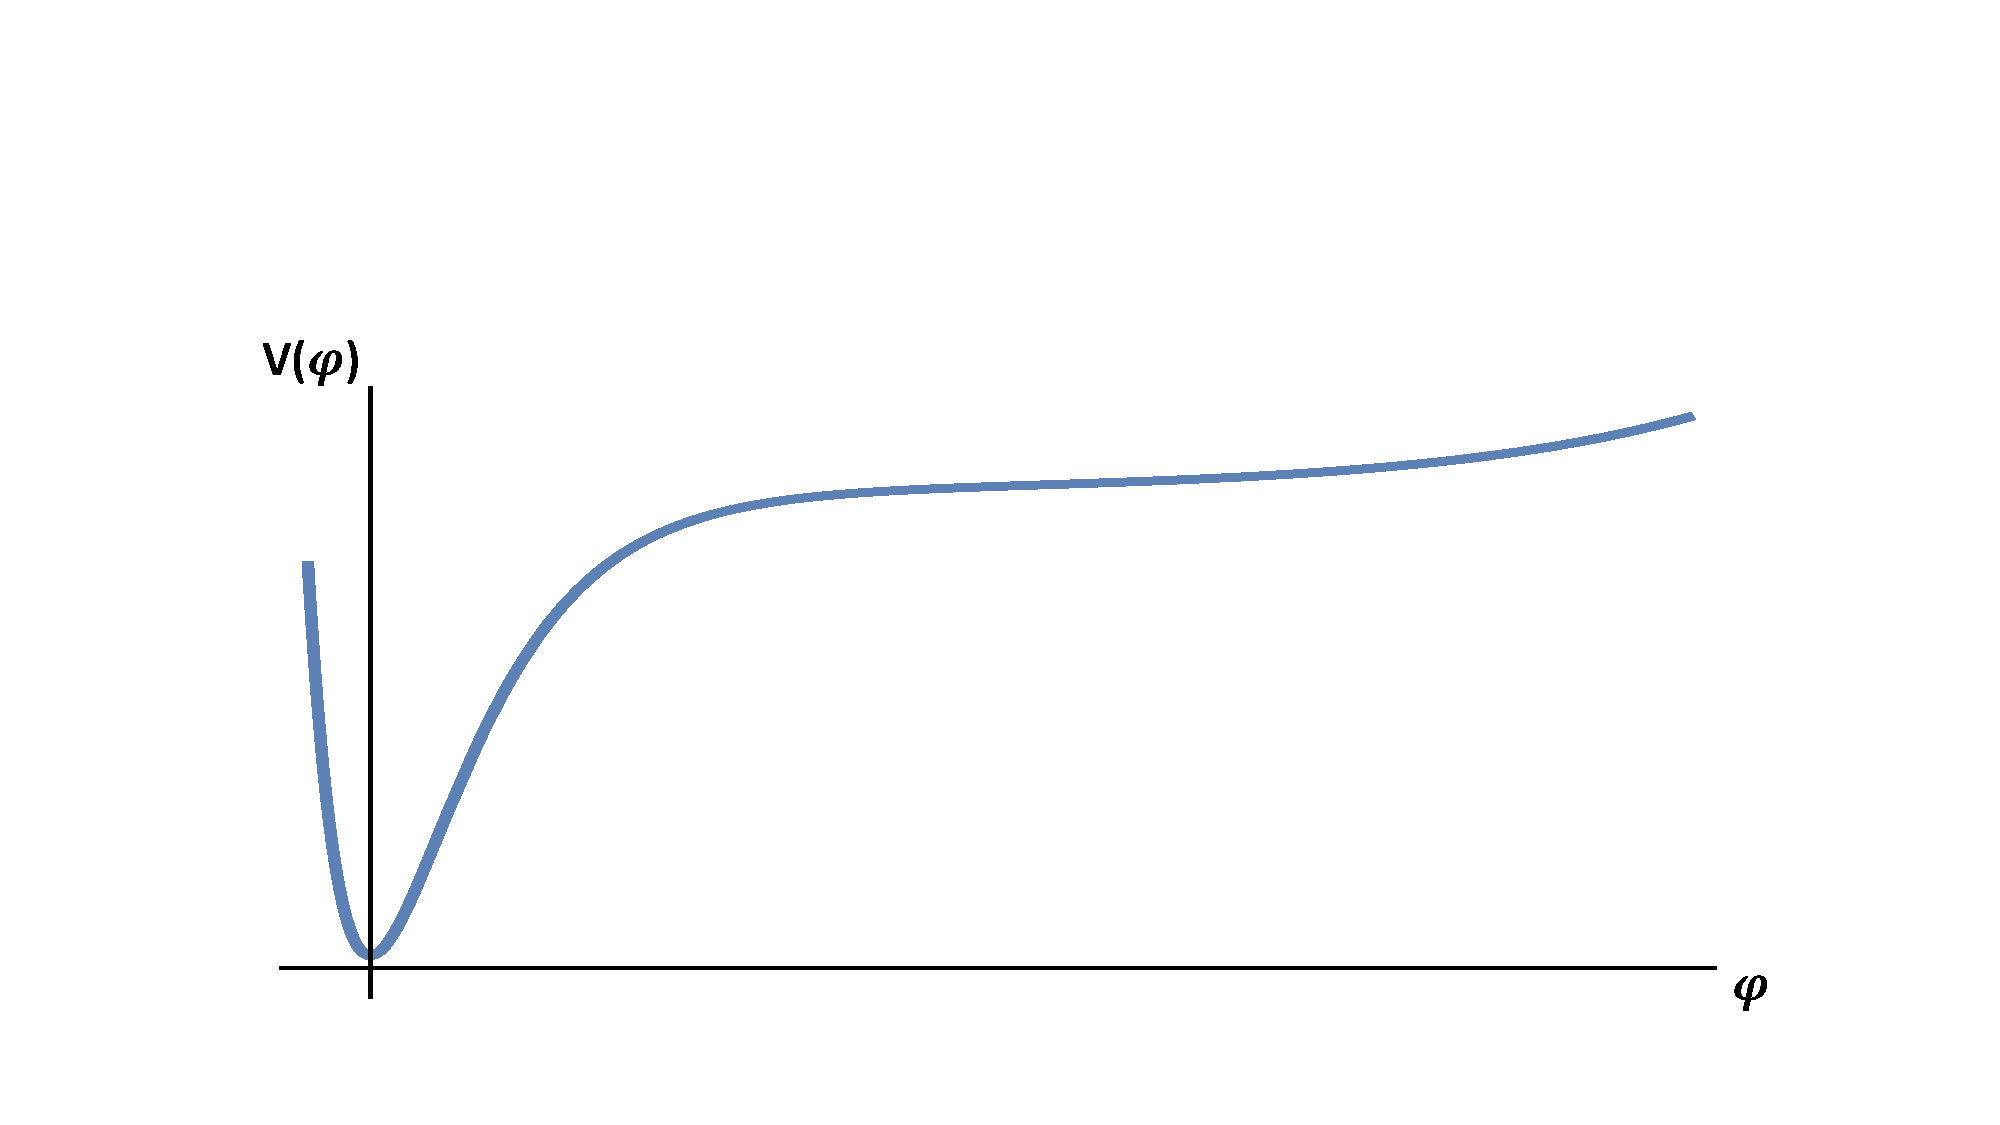
\includegraphics[width=130mm,height=80mm]{Sections/Figures/FibrePotential.pdf} 
\caption{A typical scalar potential for a fibre modulus (with all other moduli stabilised), showing a relatively large plateau with field range of order $\Delta\phi\simeq \mathcal{O}(5)\,M_{\rm Pl}$. } 
\label{Fig:Fiber} 
\end{center}
\end{figure}


\subsubsection*{Blow-up Inflation}

In this model the inflaton is the volume of a diagonal del Pezzo divisor which resolves a point-like singularity. The potential is generated by either Euclidean D3-instantons or gaugino condensation on D7-branes, and the overall volume is kept stable during inflation via the presence of additional blow-up modes\footnote{See also \cite{Krippendorf:2009zza} for a purely supersymmetric realisation of blow-up and fibre inflation in a set-up that does not need to  include an uplifting term. } \cite{Conlon:2005jm}, or logarithmic loop corrections at $\mathcal{O}(g_s^2 \alpha'^3)$ \cite{Antoniadis:2019rkh}. This is a small-field model characterised by a sub-Planckian inflaton excursion that results in a very low Hubble scale, of order $H_{\rm inf}\simeq 5\times 10^8$ GeV and a negligibly small tensor-to-scalar ratio, $r\simeq 10^{-10}$. The potential is again of the form (\ref{Refeq}) with $p=4/3$ and an effective decay constant which scales as $f \simeq M_s \simeq M_{\rm Pl}/\sqrt{\mathcal{V}}$. In fact, the potential for the canonically normalised inflaton reads (setting again $M_{\rm Pl}=1$):
\begin{equation}
\setlength\fboxsep{0.25cm}
\setlength\fboxrule{0.4pt}
\boxed{
V = V_0\left(1-\lambda \,\phi^{4/3} \,e^{-\mu\,\phi^{4/3}}\right),
}
\end{equation}
where $\lambda\sim \mathcal{V}^{5/3}$ and $\mu\sim \mathcal{V}^{2/3}$. See Fig.~\ref{Fig:BlowUp} for a 2-dimensional plot of the trajectory of Blow-up Inflation in the ($\mathcal{V}$ mode, inflaton) plane. This potential can receive large loop or higher derivative corrections that might spoil its flatness. Thus these effects need to be absent by construction or be suppressed by small coefficients. A detailed numerical analysis of inflationary solutions in the full multi-field potential was performed in \cite{Blanco-Pillado:2009dmu}, finding a robust prediction for $n_s\sim 0.96$ for $N_e=60$. A generalisation of the model including also the axionic partner of the inflaton has been presented in \cite{Bond:2006nc}. Two-field generalisations where two of the K\"ahler moduli act as inflatons were presented in \cite{Yang:2008ns,Berglund:2009uf,Kawasaki:2010ux}. In particular, the model in \cite{Kawasaki:2010ux} turns out to be a double inflation model, producing a peak in the power spectrum at observationally interesting scales.


The post-inflationary evolution of this model has been studied in detail and determines the number of efoldings of inflation which, in turn, gives the prediction for the scalar spectral index: $n_s\simeq 1-2/N_e$ \cite{Martin:2013tda}. 
After the end of inflation preheating effects cause a violent non-perturbative production of inflaton self-quanta \cite{Barnaby:2009wr} whose perturbative decay leads to the formation of a thermal bath \cite{Cicoli:2010ha,Cicoli:2010yj,Allahverdi:2020uax}. If the Standard Model lives on D7-branes wrapping the inflaton cycle, this leads to $N_e\simeq 52$ and $n_s\simeq 0.961$. Notice however that when the visible sector is sequestered from the sources of supersymmetry breaking, this initial epoch of radiation dominance can end rather quickly due to the emergence of an early matter dominated era due to the oscillations of the overall volume mode, reducing the number of efoldings to $N_e\simeq 45$ \cite{Cicoli:2016olq}.\footnote{A reduction of the number of efoldings can also be due to a very long reheating epoch from the inflaton decay when the Standard Model lives on D7-branes wrapped around a local 4-cycle which does not intersect with the inflaton blow-up mode \cite{Cicoli:2022fzy}.} The corresponding prediction for the scalar spectral index would then be $n_s\simeq 0.955$ which is in slight tension with CMB Planck data\footnote{Constraints on K\"ahler inflation models with  WMAP7 where studied in \cite{Lee:2010tk}.}\cite{Bhattacharya:2017ysa,Bhattacharya:2017pws}. Let us finally mention that an explicit embedding of this model in a globally consistent Calabi-Yau compactification with a chiral visible sector on D3-branes at singularities has been given in \cite{Cicoli:2017shd}. 


\begin{figure}[H]
\begin{center}
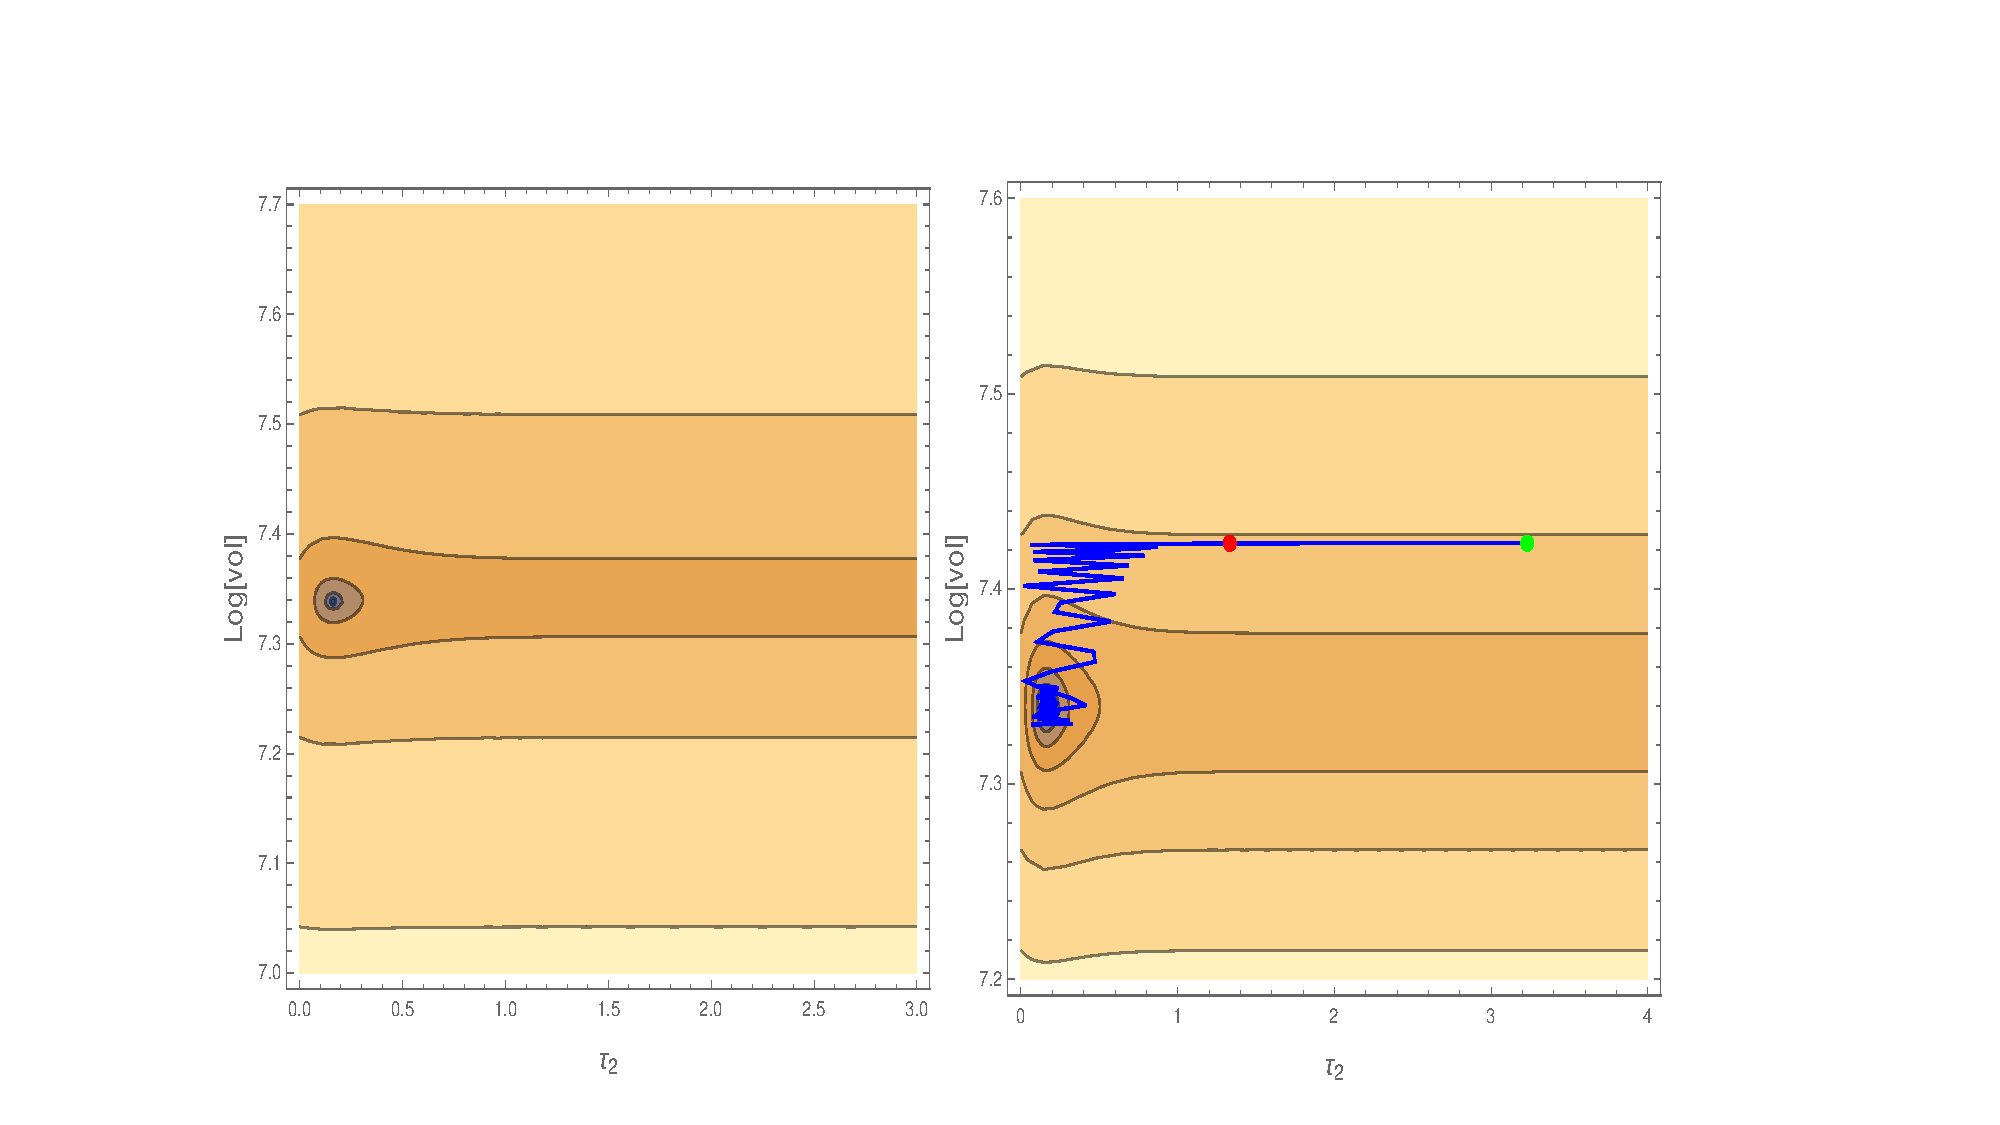
\includegraphics[width=120mm,height=85mm]{Sections/Figures/BlowUp.pdf} 
\caption{An example for the evolution trajectory of Blow-up Inflation in the ($\mathcal{V}$ mode, blow-up inflaton $\tau_2$) plane. The diagram shows level lines and the location of the global minimum. The trajectory of the inflationary field is illustrated with the green dot representing horizon exit and the red dot the end of inflation determined by $\epsilon=1$ (figure taken from \cite{Cicoli:2017shd}). The plot on the right hand side shows also the displacement of the $\mathcal{V}$ modulus during inflation.} \label{Fig:BlowUp} 
\end{center}
\end{figure}




\subsubsection*{Poly-instanton Inflation}

In this model \cite{Cicoli:2011ct} the inflaton is the volume of a so-called Wilson divisor, i.e.~a rigid divisor with a Wilson line \cite{Blumenhagen:2012kz}. This topological property implies that this divisor appears in the superpotential only via highly suppressed poly-instanton contributions \cite{Blumenhagen:2008ji} which make its potential naturally flat \cite{Cicoli:2011yy}. This potential is again of the form (\ref{Refeq}) with $p=1$ and an effective decay constant that scales as $f \simeq  M_p/\ln\mathcal{V}$. More precisely, the inflationary potential for this class of models reads:
\begin{equation}
\setlength\fboxsep{0.25cm}
\setlength\fboxrule{0.4pt}
\boxed{
V = V_0\left(1-\kappa \,\phi\,e^{-\kappa\phi}\right)\,,
}
\end{equation}
with $\kappa \simeq \ln\mathcal{V}$. The predictions of this model lie between the ones of Fibre and Blow-up Inflation. In fact, the tensor-to-scalar ratio is of order $r\simeq 10^{-5}$ together with $n_s\simeq 0.958$ at $N_e\simeq 52$. Note that explicit Calabi-Yau embeddings of this model with poly-instanton effects have been constructed in \cite{Blumenhagen:2012ue, Gao:2013hn,Lust:2013kt}. 


\subsubsection{Trigonometric Potentials from Axionic Shift Symmetries}

Closed string axions enjoy continuous shift symmetries of the type (\ref{axionshift}) which are perturbatively exact. Non-perturbative effects break them down to discrete shift symmetries. These symmetry breaking effects scale as $V_0\,e^{- i \theta}$, and the resulting scalar potential for the canonically normalised field $\phi = f \theta$ looks like:
\begin{equation}
\setlength\fboxsep{0.25cm}
\setlength\fboxrule{0.4pt}
\boxed{
V = V_0 \left[1-\cos\left(\frac{\phi}{f}\right)\right].
}
\label{AxionPot}
\end{equation}
This potential is known to give rise to accelerated expansion only for $f>M_{\rm Pl}$ (see section \ref{subsIM}). However, this result can never be achieved with control over the effective field theory since the axion decay constant scales as $f\sim M_{\rm Pl}/\tau$, where $\tau$ denotes the volume of a divisor in string units, or more in general a combination of divisors \cite{Svrcek:2006yi,Cicoli:2012sz}. Given that a fundamental requirement to trust the low-energy action is $\tau> 1$, $f$ needs to be sub-Planckian. 

A similar line of reasoning arises from the weak gravity conjecture \cite{Arkani-Hamed:2006emk} applied to axions which results in $f S \lesssim M_{\rm Pl}$ where $S$ is the instanton action. Demanding $S>1$ to keep control over the instanton expansion, implies $f<M_{\rm Pl}$, and so no inflation driven from the potential (\ref{AxionPot}). 

Let us now briefly describe the two most promising and studied way-outs to this problem.

\subsubsection*{Natural Inflation from Alignment}

This model requires at least two axions whose decay constants, even if sub-Planckian, are aligned by fine-tuning. This generates an effective trans-Planckian decay constant for the lightest eigenmode \cite{Kim:2004rp,Choi:2014rja,Kappl:2014lra}. The scalar potential of this model looks like:
\begin{equation}
\setlength\fboxsep{0.25cm}
\setlength\fboxrule{0.4pt}
\boxed{
V = \Lambda_a  \left[1-\cos\left(a_1\frac{\phi_1}{f_1}+a_2\frac{\phi_2}{f_2}\right)\right]  
+ \Lambda_b \left[1-\cos\left(b_1\frac{\phi_1}{f_1}+b_2\frac{\phi_2}{f_2}\right)\right].
}
\end{equation}
In the limit where $a_1/a_2 \to b_1/b_2$, a linear combination of the two original axions (say $\tilde{\phi}$) is flat and its decay constant $\tilde{f}$ becomes infinite. For example, for $a_1=b_1=1$ one has:
\begin{equation}
\tilde{\phi}= \frac{f_2\phi_2-a_2 f_1\phi_1}{a_2^2 f_1^2 + f_2^2}\qquad\text{and}\qquad\tilde{f}=\frac{\sqrt{a_2^2 f_1^2 + f_2^2}}{|a_2-b_2|} \xrightarrow[a_2\to b_2]{} \infty.
\end{equation}
The predictions for the main cosmological observables depend crucially on the value of $\tilde{f}$. Taking again $N_e\simeq 52$ as benchmark point, $r\lesssim 0.1$ requires $\tilde{f}\lesssim 8$. For $\tilde{f}=8$ we obtain $n_s\simeq 0.960$ and $r\simeq 0.098$. Larger values of $\tilde{f}$ are in tension with present bounds on $r$, while smaller values of $\tilde{f}$ yield a scalar spectral index which tends to be too low. The effective field theory is also marginally under control and it is rather hard to build explicit Calabi-Yau orientifold models which are globally consistent due to the need to rely on large ranks for the condensing gauge groups. Interesting models have however been proposed using combinations of $C_0$, $C_2$ and $C_4$ axions \cite{Higaki:2014pja,Ben-Dayan:2014zsa,Long:2014dta,Gao:2014uha,Li:2014lpa,Ben-Dayan:2014lca, Abe:2014xja, Angus:2021jpr}. A survey on axion inflation in  type IIB string theory compactifications and the possibility of  enlarging the field range via alignment was performed in \cite{Long:2016jvd}. They determined an upper bound on the inflationary field range of $\Delta\phi \lesssim 0.3\Mp$. 



\subsubsection*{N-flation}

This scenario involves several axions, each of them with a sub-Planckian decay constant, whose collective motion however results in an effective trans-Planckian decay constant \cite{Dimopoulos:2005ac}. The simplest version of this model features a scalar potential of the form:
\begin{equation}
\setlength\fboxsep{0.25cm}
\setlength\fboxrule{0.4pt}
\boxed{
V=\sum_{i=1}^N \Lambda \cos\left(\frac{\phi_i}{f}\right) \simeq \frac12 \left(\frac{\Lambda^2}{f}\right)^2 \sum_{i=1}^N \phi_i^2\,,
}
\end{equation}
where we have approximated the potential around the minimum. An initial displacement of each axion of order $f$ generates an overall displacement of the radial field $\rho= \sqrt{\sum_{i=1}^N \phi_i^2}$ of order $f_{\rm eff}=\sqrt{N}\,f$. Slow-roll inflation can then be easily achieved for $N\gg 1$. The predictions for the main cosmological observable are very similar to the ones of Natural Inflation: $n_s\simeq 0.96$ and $r\simeq 0.1$, with $r$ in tension with data \cite{Kim:2011jea}. Moreover, obtaining $\mathcal{O}(50)$ efoldings of inflation and matching the observed amplitude of scalar fluctuations requires a very large number of axions, $N\gtrsim 10^5$, and a relatively small Calabi-Yau volume $\mathcal{V}\simeq 10^3$. This implies that the stabilisation of the corresponding saxions at perturbative level is hardly under control \cite{Cicoli:2014sva}. In addition, all these light species can contribute to the renormalisation of the Planck mass.  Attempts to embed N-flation in string theory have been proposed in \cite{Easther:2005zr,Grimm:2007hs,Cicoli:2014sva,Grimm:2014vva} 



\subsubsection{Power-law Potentials from Axionic Shift Symmetries}

Several scenarios corresponding to large field inflation have been proposed using string theoretical axions (historically, several of these were motivated by the claimed observation of primordial tensor modes by the BICEP collaboration \cite{BICEP}). In principle, these offer
the attractive possibility of both minimising fine tuning through an underlying shift symmetry while also offering the chance to compare with observations on relatively short time-scales.
 
\subsubsection*{Axion Monodromy}

Another scenario of large field inflation driven by closed string axions is Axion Monodromy (AM) where the axionic shift symmetry is broken at tree-level. In this case the resulting inflationary potential is power-law \cite{Silverstein:2008sg,McAllister:2008hb}. 

The original model is characterised by a linear potential, with two main scenarios depending on the nature of the axion: 
\begin{itemize}
\item \text{$B_2$-axion monodromy}: Inflation is driven by the $B_2$-axion $b$ whose potential originates from the reduction of the DBI action of a D5-brane wrapped around a 2-cycle $\Sigma_2$:
\begin{equation}
\setlength\fboxsep{0.25cm}
\setlength\fboxrule{0.4pt}
\boxed{
V (b) = V_0 \sqrt{{\rm Vol}(\Sigma_2) + b^2} \simeq \mu^3 \frac{\phi}{f}\,,
}
\end{equation}
where we have expanded for large values of $b$ and we have canonically normalised.

\item \text{$C_2$-axion monodromy}: Inflation is driven by the $C_2$-axion $c$ whose potential originates from the reduction of the DBI action of an NS5-brane wrapped around a 2-cycles $\Sigma_2$:
\begin{equation}
\setlength\fboxsep{0.25cm}
\setlength\fboxrule{0.4pt}
\boxed{
V (c) = V_0 \sqrt{{\rm Vol}(\Sigma_2) + g_s^2 c^2} \simeq \mu^3 \frac{\phi}{f}\,,
}
\label{VAxMon}
\end{equation}
where we have expanded for large values of $b$ and we have canonically normalised.
\end{itemize}
Note that, given that the $B_2$-axion appears in the K\"ahler potential $K = -3\ln\left(T+\bar{T}+\gamma b^2\right)$, axion monodromy models where the inflaton is $b$ are affected by the $\eta_V$-problem. This is not true for the case of the $C_2$-axion $c$, which is therefore the most promising candidate to drive axion monodromy. Note that this model is affected by backreaction effects \cite{Conlon:2011qp, Valenzuela:2016yny}, which may be addressed by using bifurcated throats \cite{Retolaza:2015sta}. 
%
See also \cite{Andriot:2015aza} for a no-go theorem on embedding  the original axion monodromy inflation mechanism of \cite{Silverstein:2008sg} in a concrete compactification.

In terms of observational consequences, this model yields $n_s\simeq 0.971$ and $r\simeq 0.083$ at $N_e\simeq 52$, with large tensor modes in tension with data. A potential way-out to reduce the tensor-to-scalar ratio relies on flattening effects which could make the inflationary potential shallower due to an appropriate interaction of the inflaton with heavy field which have been integrated out \cite{Dong:2010in}.    A qualitative picture of this mechanism is shown in Fig.~\ref{Fig:Flattening}. A further source of flattening, arising from fluxes, was analysed in \cite{Landete:2017amp} in the context of type IIB/F-theory flux compactifications with mobile 7-branes, which allowed for $0.14 \gtrsim r \gtrsim 0.04$.

Moreover, a cosine modulation of the scalar potential (\ref{VAxMon}) generated by non-perturbative effects, can yield oscillations in the scalar power-spectrum \cite{Flauger:2009ab,Peiris:2013opa} and resonant non-Gaussianities \cite{Hannestad:2009yx}. Depending on the size of the modulations, these can  change the background evolution allowing successful inflation for smaller field ranges in axion monodromy and sub-Planckian decay constants in a modulated axion inflation \cite{Parameswaran:2016qqq}. Modulated potentials also have interesting phenomenology such as the production of abundant primordial black holes, which can form all or part of the dark matter \cite{Ozsoy:2018flq}. More general expressions for the potential of axion monodromy are:
\begin{equation}
\setlength\fboxsep{0.25cm}
\setlength\fboxrule{0.4pt}
\boxed{
V = \mu^{4-p} \left(\frac{\phi}{f}\right)^p \,,
}
\end{equation}
where $p$ can be either $p=2/3$ \cite{Silverstein:2008sg} of $p=2$ \cite{Kaloper:2008fb,Berg:2009tg,Palti:2014kza}. 


\begin{figure}[t]
\begin{center}
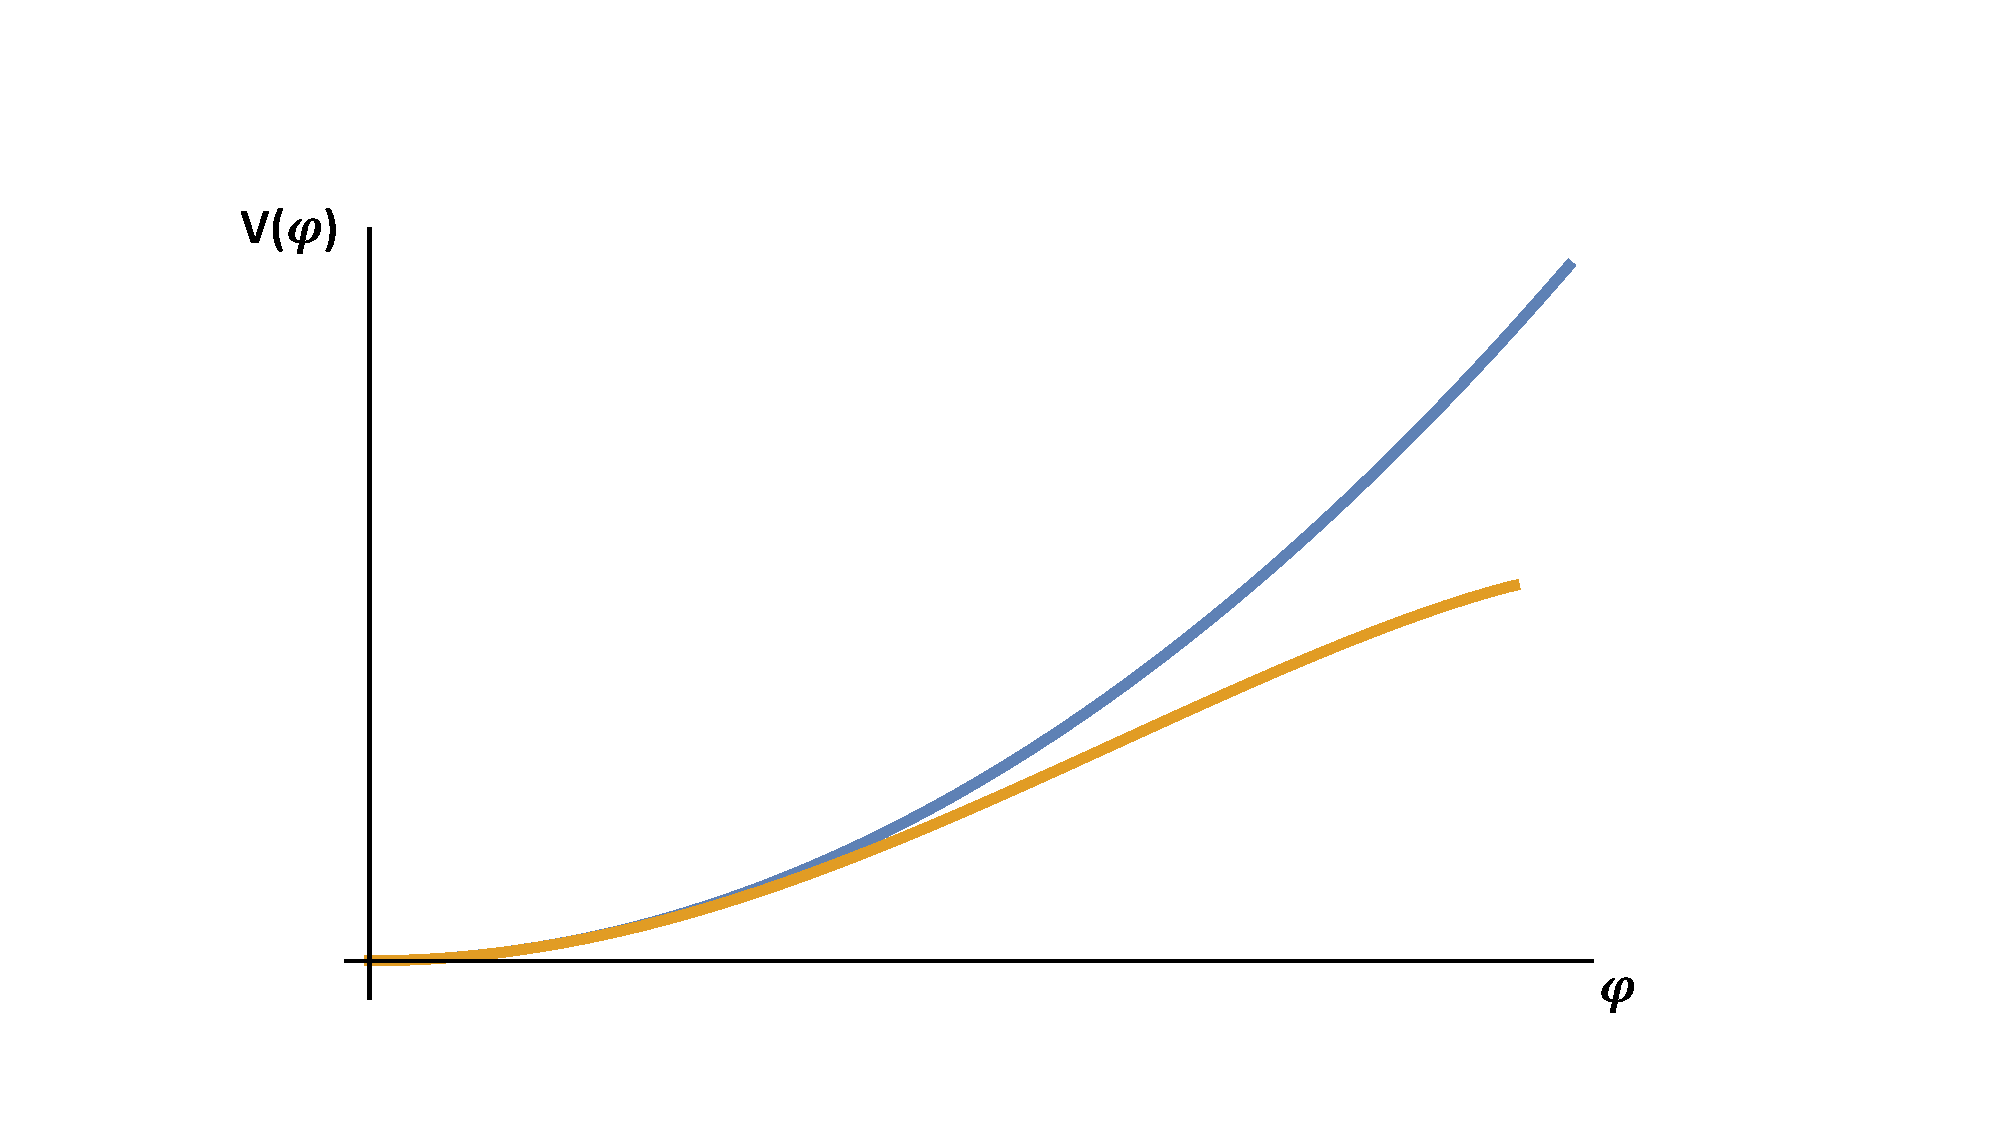
\includegraphics[width=140mm,height=80mm]{Sections/Figures/FlatteningPotential.pdf} 
\caption{An example for a power law potential as appearing in Axion Monodromy or Alignment proposals. Here the simplest case of a quadratic potential is shown together with a flattening mechanism that modifies the corresponding potential after introducing couplings with heavy moduli fields.} 
\label{Fig:Flattening} 
\end{center}
\end{figure}


\subsubsection*{F-term Axion Monodromy}

An alternative axion monodromy mechanism was introduced in \cite{Marchesano:2014mla,Blumenhagen:2014gta,Hebecker:2014eua}. In this proposal, the idea is that the same background fluxes used for moduli stabilisation already generate a tree-level F-term scalar potential for the axion. The shift symmetry of the axion is broken by the background  fluxes to generate a non-oscillatory term in the potential, leading to diverse inflaton potentials, including linear large field behaviour, chaotic inflation, as well as potentials with even higher powers. Therefore, the potentials take the form 
\be
 V \sim A + B\, \theta^2 +C\, \theta \cos(\theta) +\dots \, ,
 \ee
 where $\theta$ is the axion  and $A, B$ depend on  other moduli and the fluxes, and the dots include further mixed terms, including sines and cosines multiplied by powers of $\theta$ \cite{Flauger:2014ana,Kobayashi:2015aaa,CaboBizet:2016uzv}. As mentioned before,  subleading (but sufficiently large) modulations can superimpose periodically steep cliffs and gentle plateaus onto the underlying potential. This can allow sufficient efolds of inflation with smaller field ranges lowering the tensor-to-scalar ratio, even achieving natural inflation with sub-Planckian axion decay constants \cite{Parameswaran:2016qqq,Kadota:2016jlw,Ozsoy:2018flq}. Realisations of this mechanism using different open and closed string axions can be found in \cite{Ibanez:2014kia,Franco:2014hsa,Hayashi:2014aua,Ibanez:2014swa,Garcia-Etxebarria:2014wla,Escobar:2015fda,Escobar:2015ckf,Hebecker:2015tzo,CaboBizet:2016uzv,Landete:2016cix}. 
The consistency of this new scheme with moduli stabilisation was analysed in \cite{Blumenhagen:2014nba,Hebecker:2014kva} and \cite{Blumenhagen:2015kja,Blumenhagen:2015qda,Blumenhagen:2015xpa} in the context of non-geometric flux compactifications.\footnote{See \cite{Damian:2018tlf} for a two field analysis of the models in \cite{Blumenhagen:2015kja}.} Further constraints have been analysed in \cite{Landete:2017amp,Kim:2018vgz}.

\subsubsection*{D7-Brane Inflation}

D7-deformation moduli enjoy an approximate shift symmetry at large complex structure which can be used to protect the inflaton potential. This can allow for stringy realisations of both large and small field models of inflation. In the large field case, the symmetry is broken by three-form fluxes which can develop a tunable scalar potential of the typical chaotic inflation form \cite{Hebecker:2014eua}:
\begin{equation}
\setlength\fboxsep{0.25cm}
\setlength\fboxrule{0.4pt}
\boxed{
V = \frac{m^2}{2}\,\phi^2\,.
}
\end{equation}
Such a model however predicts an amplitude of tensor modes above present observational bounds. 

On the other hand, small field models of inflation can be developed by focusing on systems of D7-branes wrapped around two different representative of the same family of 4-cycles which intersect over a 2-cycle with non-zero gauge flux. This gauge flux generates a force between the D7-branes that attracts them. This scenario is called Fluxbrane Inflation and gives rise to the following D-term inflationary potential for the relative position of the two D7-branes \cite{Hebecker:2011hk,Hebecker:2012aw,Arends:2014qca}:
\begin{equation}
\setlength\fboxsep{0.25cm}
\setlength\fboxrule{0.4pt}
\boxed{
V = V_0\left(1+\alpha\ln\left(\frac{\phi}{\phi_0}\right)\right),    
}
\end{equation}
with $\alpha\simeq g_{\rm YM}^2/(16\pi^2)\ll 1$. For our benchmark point $N_e\simeq 52$, this potential yields $n_s\simeq 1-1/N_e\simeq 0.981$ which is in slight tension with CMB data. Moreover the tensor-to-scalar ratio is $r\simeq 4\alpha/N_e \simeq 5\times 10^{-6}$ for $g_{\rm YM}\simeq 0.1$. 


\subsubsection*{Wilson Line Inflation}

The T-dual picture of inflation models based on branes at angles \cite{Garcia-Bellido:2001lbk,Blumenhagen:2002ua,Gomez-Reino:2002yja} is Wilson Line Inflation, as branes intersecting at angles are dual to magnetised branes and brane deformation moduli are dual to Wilson line moduli. Ref \cite{Avgoustidis:2006zp} presented a model of inflation driven by Wilson line moduli including moduli stabilisation. The scalar potential in the small field regime takes the form:
\begin{equation}
\setlength\fboxsep{0.25cm}
\setlength\fboxrule{0.4pt}
\boxed{
V = A- \frac{B}{\phi^2}\,,
}
\end{equation}
leading to the following predictions for the two main cosmological observables at $N_e\simeq 52$: $n_s\simeq 0.971$ and $r\simeq 10^{-8}$. Note that larger values of the tensor-to-scalar ratio can be obtained in models of warped Wilson Line DBI Inflation \cite{Avgoustidis:2008zu,Kooner:2015rza}.

\subsubsection{Potentials in the Absence of Explicit Symmetries}

Several string inflationary models do not enjoy an underlying UV symmetry which protects the inflationary potential against large quantum correction. However, one can still build a working inflationary model if the system allows for enough tuning freedom to suppress all dangerous corrections to the inflationary potential. We shall now briefly discuss the main classes of string models of inflation which are not based on any symmetry.

\begin{figure}[t]
\begin{center}
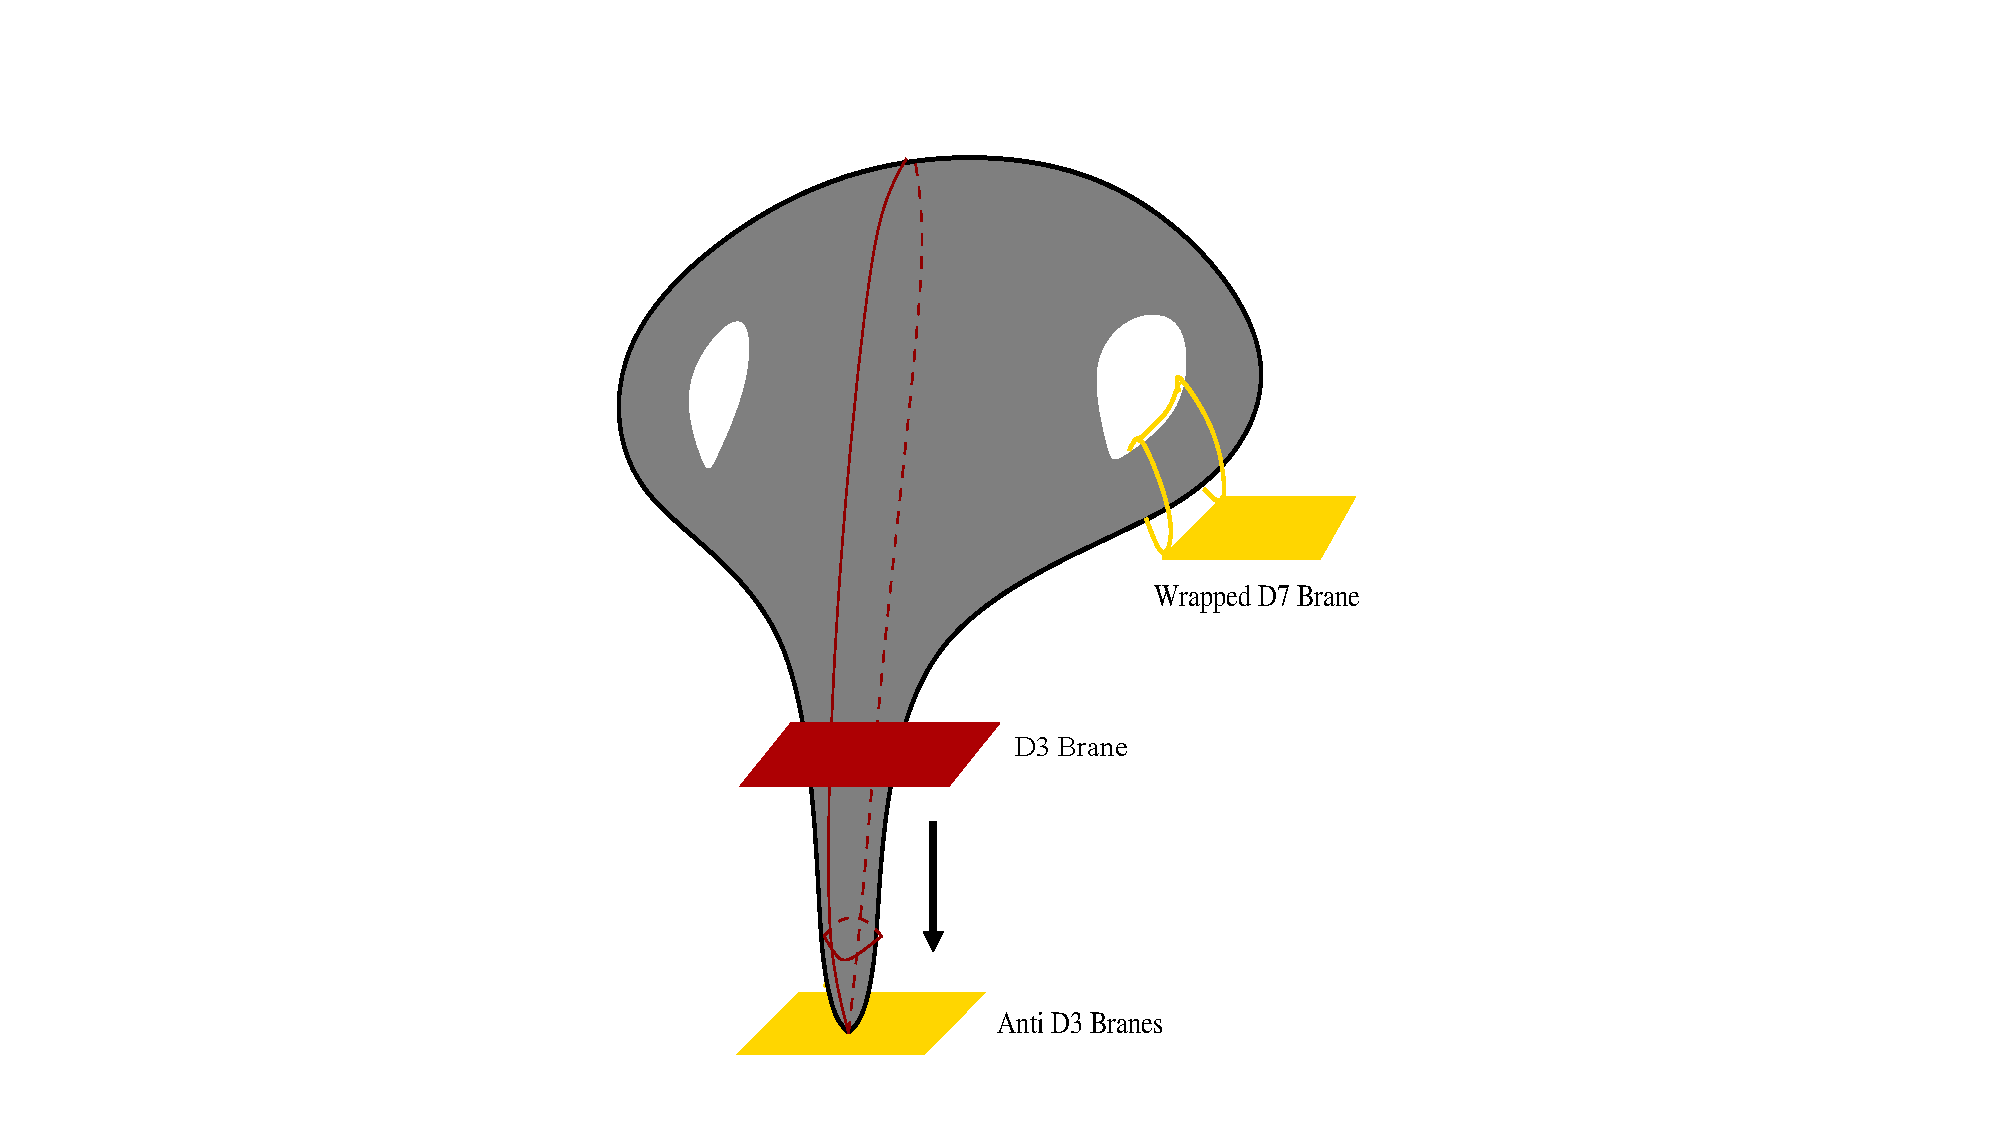
\includegraphics[width=130mm,height=80mm]{Sections/Figures/BraneInflation.pdf} 
\caption{Warped brane-antibrane inflation. The set-up of KKLT is simply complemented with a moving D3 brane that is attracted to the anti-brane at the tip of a warped throat. In principle the warping allows for naturally small $\epsilon, \eta$ parameters. However, if, as in KKLT and LVS, moduli are fixed non-perturbatively then there are extra contributions to $\eta_V$ of order $\mathcal{O}(1)$ illustrating the single-field $\eta_V$ problem.} 
\label{Fig:KKLMMT} 
\end{center}
\end{figure}

\subsubsection*{{\rm D3}-$\overline{\rm D3}$ Inflation}

One of first attempts to realise inflation in string theory has used the separation between branes as the field which drives inflation \cite{Dvali:1998pa}. Since D-branes are BPS states their separation is a modulus with no potential. However if instead of two D-branes there are D-branes and anti D-branes there is a Coulomb attraction that gives rise to a scalar potential for the brane separation \cite{Burgess:2001fx,Dvali:2001fw}. More precisely, the model is based on a D3-$\overline{{\rm D3}}$ brane system where the inflaton is the open string modulus controlling the distance between the D3 and the $\overline{{\rm D3}}$ brane which move towards each other \cite{Burgess:2001fx,Dvali:2001fw}. For general studies of the dynamics of D-brane systems see e.g.~\cite{Burgess:2003qv, Burgess:2003mm, Burgess:2003tz, Easson:2007fz}. In \cite{Kachru:2003sx} these configurations were considered including warped compactifications in which warping can be used to get slow-roll (see Figure \ref{Fig:KKLMMT} for a cartoon of the warped brane-antibrane inflation set-up). The Coulomb potential for systems of D3-$\overline{{\rm D3}}$ branes in warped compactifications reads \cite{Kachru:2003sx}:
\begin{equation}
\setlength\fboxsep{0.25cm}
\setlength\fboxrule{0.4pt}
\boxed{
V = V_0 \left(1-\lambda\, \frac{V_0}{\phi^4}\right),
}
\label{Vbraneinfl}
\end{equation}
where the overall scale of the potential is set by the warped $\overline{{\rm D3}}$-brane tension: $V_0 \simeq T_3\,e^{4 A(r_{\rm IR})}$. Contrary to the original proposal in which the parameters of the potential do not give naturally small slow-roll parameters, 
the advantage of warping is that $V_0 \propto e^A$ can be as small as we want and both $\eta_V$ and $\epsilon$ can be as small as we want with $\epsilon \propto \eta_V^2 \ll \eta_V$. The predictions for the main cosmological observables evaluated at $N_e\simeq 52$ are $n_s\simeq 0.968$ and $r\simeq 7\times 10^{-8}$ \cite{Ma:2013xma}. 
This indicates that this is a small-field model,  in agreement with the microscopic bound on the field range for D3-brane inflation discussed in \cite{Baumann:2006cd}.  The field range can be slightly increased if  inflation is driven by the motion of a D5-brane wrapping an $2$-cycle \cite{Becker:2007ui}. In this model though, backreaction of the D5-brane needs to be checked. Furthermore, a D5-brane natural inflation model, was proposed in \cite{Kenton:2014gma}, where the D5-brane moved along an  angular direction in a warped resolved conifold \cite{PandoZayas:2000ctr,Klebanov:2007us}. The challenge in this model is to ensure that it is consistent with moduli stabilisation. 

In the original formulation of \cite{Burgess:2001fx,Dvali:2001fw} a crucial assumption of this model was that the dynamics which stabilises the K\"ahler moduli in the bulk does not alter the flatness of the potential (\ref{Vbraneinfl}) since at the time of the proposal there was no explicit scenario of moduli stabilisation. This is generically not the case since inflaton-dependent higher dimensional operators arise from both the tree-level K\"ahler potential and the prefactors of non-perturbative effects \cite{Kachru:2003sx}. A detailed study of how moduli stabilisation can be incorporated in this set-up has been reviewed in \cite{Baumann:2014nda} (crucial as including moduli stabilisation substantially changes the dynamics of the original proposal). See however a recent potential way-out exploiting perturbative stabilisation mechanism via RG effects \cite{Burgess:2022nbx} for which the warped inflation potential is at work even after moduli stabilisation.

One of the attractive points of D3-$\overline{{\rm D3}}$ inflation is the fact that the dimensionality of spacetime may play a role. In fact ref. \cite{Burgess:2001fx} proposed that in a gas of branes, D3-branes (for the type IIB case) are such that they can meet in 10 dimensions. This idea was further explored in \cite{Karch:2005yz, Durrer:2005nz}. Furthermore, the ending of brane inflation via the string tachyon is a stringy way to end inflation in a string theory realisation of hybrid inflation. The idea is that, while the branes approach each other, there is an open string state stretching between the two branes that gets lighter and lighter, at a critical distance becomes massless and, after that, becomes tachyonic. The end of inflation is the point where the tachyon reaches a minimum of its potential, which is essentially of the Mexican hat shape. This leads, in turn, to the prediction after inflation of cosmic strings (D1-branes) that may be one of the very few observable implications of 
string cosmology which is directly stringy in nature \cite{Sarangi:2002yt,Copeland:2003bj}.

D3-$\overline{{\rm D3}}$ inflation also offers the cleanest illustration of one of the more distinctive possibilities within \emph{string} inflation: the disappearance of the inflaton field at the end of inflation. The inflaton is the position modulus of the D3-brane, but after brane-antibrane annihilation this field is entirely removed from the effective field theory. This is in contrast to most field theory scenarios where, although the inflaton may decay, the field remains present in the theory.

\subsubsection*{Inflection Point Inflation}

Ref. \cite{Baumann:2007np,Baumann:2007ah,Krause:2007jk} have shown that the single-field $\eta_V$-problem of D3-$\overline{{\rm D3}}$ Inflation can be avoided since this system features enough tuning freedom to suppress dangerous Planck-suppressed higher dimensional operators that would generate corrections to the inflaton mass of order the Hubble constant during inflation.  

In the Kuperstein embedding, one has two contributions to the slow-roll $\eta_V$-parameter with opposite signs which can ensure $\eta_V\ll 1$, inducing inflation near an inflection point where the potential can be rewritten as an expansion as:
\begin{equation}
\setlength\fboxsep{0.25cm}
\setlength\fboxrule{0.4pt}
\boxed{
V \simeq V_0 \left(1+ \lambda_1 \frac{\phi}{M_{\rm Pl}} + \lambda_3 \frac{\phi^3}{M_{\rm Pl}^3} + \cdots \right) \, .
}
\end{equation}
This model is in slight tension with CMB observations since the prediction of the scalar spectral index depends on the total number of efoldings $N_e^{\rm tot}$. If $N_e^{\rm tot}\lesssim 120$, $n_s\gtrsim 1$, while $n_s\simeq 1-4/N_e$ only if $N_e^{\rm tot} \gg 2 N_e$. In this regime, $n_s\simeq 0.923$ for $N_e\simeq 52$ \cite{Linde:2007jn}, requiring a very large total number of efoldings which is however disfavoured by statistical considerations \cite{Agarwal:2011wm,McAllister:2012am}. Moreover, being a small-field model, the tensor-to-scalar ratio is negligible: $r\lesssim 10^{-6}$. For realisations
of inflection points in other settings see e.g \cite{Ben-Dayan:2013fva, Blanco-Pillado:2012uao, Maharana:2015saa}.


\subsubsection*{D3-D7 Inflation}

In cases without warping, inflation can occur in D3-D7 systems where the inflaton is a D3-brane position modulus whose D-term potential is generated by non-zero gauge fluxes on D7-branes which break supersymmetry. In order to stabilise the compact extra dimensions, the K\"ahler moduli can be frozen by gaugino condensation on D7-branes leading to extra contributions to the inflationary potential due to the mixing between K\"ahler and D3-position moduli in the K\"ahler potential. The final expression for the inflationary potential looks like \cite{Dasgupta:2002ew,Dasgupta:2004dw,Burgess:2008ir}: 
\begin{equation}
\setlength\fboxsep{0.25cm}
\setlength\fboxrule{0.4pt}
\boxed{
V = V_0 + A\,\ln\phi -\frac{m^2}{2}\, \phi^2+\frac{\lambda}{4}\,\phi^4\,.
}
\end{equation}
Defining $\alpha\equiv 2 m^2/V_0$ the prediction for the scalar spectral index is:
\begin{equation}
n_s=1-\alpha\left(1+\frac{1}{1-e^{-\alpha N_e}}\right)\simeq 1-\frac{1}{N_e} \quad\text{for}\quad \alpha \to 0\,.
\end{equation}
For $N_e\simeq 52$ and $\alpha\to 0$, this gives $n_s\simeq 0.981$ which is too blue. A value for $n_s$ compatible with Planck data ($n_s\simeq 0.966$) can be obtained for $\alpha\sim\mathcal{O}(0.01)$, leading however to a tension with current bounds on cosmic strings \cite{Haack:2008yb}. The tensor-to-scalar ratio turns out to be rather small once perturbativity and consistency with cosmic string bounds is required: $r\lesssim 10^{-6}$.

\subsubsection*{M5-brane inflation} 

In the context of M-theory compactifications \cite{Horava:1995qa,Horava:1996ma,Witten:1996mz}, an inflationary scenario was proposed, where the inflaton corresponds to the position of one or more M5-branes, moving along the interval. Inflation then comes to an  end as the M5-branes collide with and dissolve through small instanton transitions \cite{Buchbinder:2004nt,Becker:2005sg,Krause:2007jr}. The challenge in this scenario is to achieve a suitable inflationary potential, while simultaneously stabilising the geometric moduli. 

\subsubsection*{Racetrack Inflation}

Saddle point inflation can also be realised by an appropriate choice of the underlying parameters for a $C_4$-axion in the so-called Racetrack Inflation scenario which is characterised by a superpotential of the form \cite{Blanco-Pillado:2004aap,Blanco-Pillado:2006dgl}:
\begin{equation}
\setlength\fboxsep{0.25cm}
\setlength\fboxrule{0.4pt}
\boxed{
W = W_0 + A\,e^{-a T} + B\,e^{-b T}\,.
}
\end{equation}
Inflation takes place mainly along the axionic direction given by ${\rm Im}(T)$, however the saxion ${\rm Re}(T)$ also evolves. This model requires a contrived choice of underlying parameters with an inflationary trajectory which might be spoiled by quantum corrections (such as, for example, $\alpha'$ effects) that can either destabilise ${\rm Re}(T)$ or make the potential steeper along the ${\rm Im}(T)$-direction \cite{Greene:2005rn}. This is a small-field model which, in the original formulation of \cite{Blanco-Pillado:2004aap}, predicts $n_s\simeq 0.942$ and $r\lesssim 10^{-8}$ for our benchmark point $N_e\simeq 52$. 

\subsubsection*{Volume Modulus Inflation}

As we have already pointed out, the overall volume modulus of type IIB string compactifications $\mathcal{V}$ does not enjoy an approximate rescaling symmetry since the leading order $\alpha'^3$ effect that breaks the no-scale structure depends explicitly on $\mathcal{V}$. However, if enough tuning freedom is present, also the volume mode can also be used to drive inflation near an inflection point induced by at least 5 different contributions to its scalar potential. These can arise from $\alpha'$ effects, $g_s$ loops, higher F-terms, $\overline{D3}$-brane contribution and D-terms. The resulting scalar potential for the canonically normalised inflaton looks like \cite{Cicoli:2015wja} (see also \cite{Antoniadis:2020stf}):
\begin{equation}
\setlength\fboxsep{0.25cm}
\setlength\fboxrule{0.4pt}
\boxed{
V = V_0 \left(\kappa_{\alpha'}\,e^{-\sqrt{\frac{27}{2}}\phi}-\kappa_{g_s}\,e^{-\frac{10}{\sqrt{6}}\phi}-\kappa_{F^4}\,e^{-\frac{11}{\sqrt{6}}\phi}
+\kappa_{\bar{D3}}\,e^{-\sqrt{6}\phi}+\kappa_D\,e^{-\frac{8}{\sqrt{6}}\phi}\right),
}
\label{Vpot}
\end{equation}
where all the $\kappa$'s are flux-dependent $\mathcal{O}(1)$ coefficients. An example showing an inflection point around $\phi\simeq \mathcal{O}(7)$ and a late time minimum at $\phi\simeq \mathcal{O}(24)$ is shown in Fig. \ref{Fig:VolInfl}. Due to the large tuning freedom, this model can reproduce the observed value of the scalar spectral index but tensor modes are unobservable, as in any inflection point inflation model.

These models are particularly interesting to reconcile high scale inflation with low energy supersymmetry \cite{Conlon:2008cj}, as a potential solution to the tension pointed out in \cite{Kallosh:2004yh}. In fact, in any viable model the inflationary energy density should not exceed the height of the barrier towards decompactification, otherwise the volume mode would run-away to infinity:
\begin{equation}
H_{\rm inf}^2 M_{\rm Pl}^2 \lesssim V_{\rm barrier}\,.
\end{equation}
In KKLT and LVS models, this sets therefore the following bounds:
\begin{eqnarray}
V_{\rm barrier}^{({\rm KKLT})} &\sim& m_{3/2}^2 M_{\rm Pl}^2\quad\Rightarrow\quad H_{\rm inf}\lesssim m_{3/2}\,, \\
V_{\rm barrier}^{({\rm LVS})} &\sim& m_{3/2}^3 M_{\rm Pl}\quad\Rightarrow\quad H_{\rm inf} \lesssim m_{3/2} \sqrt{\frac{m_{3/2}}{M_{\rm Pl}}}\,.
\end{eqnarray}
Given that in a supergravity framework the mass of the supersymmetric partners is generically of order $m_{3/2}$, a high value of $H_{\rm inf}$ necessarily implies high scale supersymmetry. Two solutions rely on decoupling the height of the barrier from the soft terms $M_{\rm soft}$: ($i$) by tuning the scalar potential so that $V_{\rm barrier}$ becomes independent of $m_{3/2}$ as in racetrack models \cite{Kallosh:2004yh}, or ($ii$) by sequestering the sources of supersymmetry breaking from the visible sector so that $M_{\rm soft}\ll m_{3/2}$ \cite{Blumenhagen:2009gk,Aparicio:2014wxa}. Another possibility would instead be to exploit the fact that the gravitino mass is $\mathcal{V}$-dependent since $m_{3/2}^2 = e^K |W|^2$ with $K=-2\ln\mathcal{V}$. Hence, if inflation is driven by a rolling $\mathcal{V}$ mode with a potential similar to (\ref{Vpot}), the gravitino mass during inflation could be much higher than today. Being necessarily a small field model with a sub-Planckian field range, the tensor-to-scalar ratio is however very small, $r\lesssim 10^{-9}$, and so TeV-scale supersymmetry can be made compatible at most with $H_{\rm inf}\lesssim 10^{10}$ GeV, but not higher. 

\begin{figure}[t]
\begin{center}
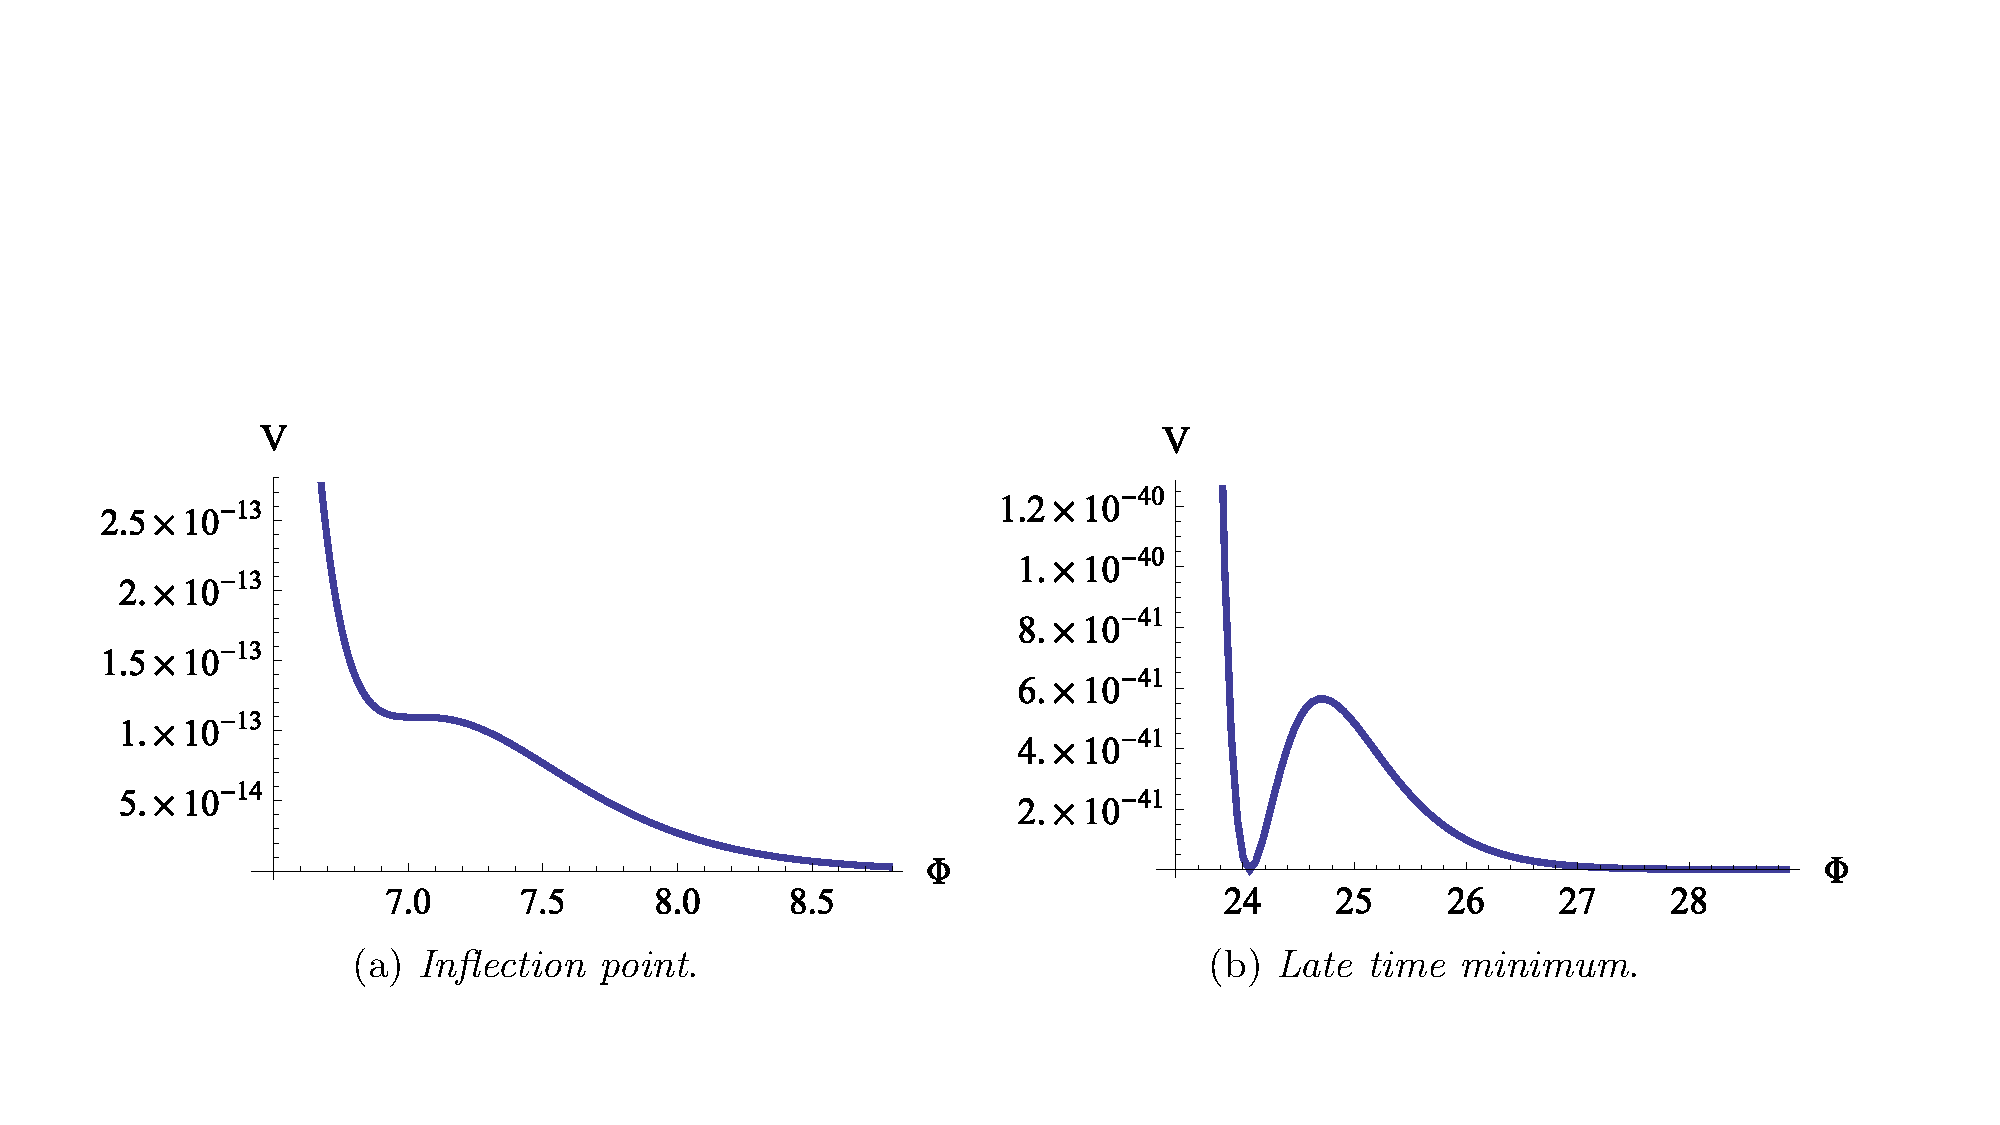
\includegraphics[width=140mm,height=85mm]{Sections/Figures/InflectionPoint.pdf} 
 \vskip -25pt
\caption{An example of  inflection point inflation for  volume modulus inflation  (figure taken from \cite{Cicoli:2015wja}). } 
\label{Fig:VolInfl} 
\end{center}
\end{figure}


\subsubsection*{DBI Inflation}

Accelerated expansion can also be achieved beyond the slow-roll approximation by exploiting the relativistic dynamics of spacetime-filling D-branes moving in a warped throat \cite{Alishahiha:2004eh,Silverstein:2003hf}. This is the so-called DBI inflation scenario characterised by non-canonical kinetic terms arising from the DBI action and a Lagrangian density of the form:
\begin{equation}
\setlength\fboxsep{0.25cm}
\setlength\fboxrule{0.4pt}
\boxed{
\mathcal{L} = - T(\phi) \left(\sqrt{1+\frac{(\partial \phi)^2}{T(\phi)}}-1\right)-V(\phi)\,,
\label{LDBI}
}
\end{equation}
where $\phi$ is the D-brane position modulus and $T(\phi)$ is the warped tension of the D-brane. The functional form of $T(\phi)$ and the potential depends on the dimensionality of the brane and determines the phenomenology of the scenario (see e.g.~\cite{Shandera:2006ax,Bean:2007hc,Ma:2013xma}). 

In the original set-up, a D3-brane moves relativistically in a warped throat. In this case, two scenarios can arise: the so-called UV-model where the brane moves from the UV end of the throat towards its tip \cite{Alishahiha:2004eh,Silverstein:2003hf}, and the IR-model where the brane moves from the tip of the throat to its UV end \cite{Chen:2004gc,Chen:2005ad}. The scalar potentials for each case read:
\begin{equation}
V = V_{\rm UV} \sim \phi^2\qquad\text{or}\qquad V = V_{\rm IR} = V_0-\frac{\beta}{2} H^2\phi^2\,,
\end{equation}
where $\beta$ is an $\mathcal{O}(1)$ positive constant. Accelerated expansion is obtained since the non-canonical form of the kinetic terms forces a speed limit on the motion of the D3-brane, under the assumption that quantum and backreaction effects do not modify the form of the Lagrangian (\ref{LDBI}). 
Besides D3-branes, DBI inflation driven by the relativistic motion of  D5- and D7-branes  in a warped throat has been studied in \cite{Kobayashi:2007hm}. Furthermore, just as in the non-relativistic case, also in this case, DBI inflation can be driven by warped Wilson lines, as studied in \cite{Avgoustidis:2008zu,Kooner:2015rza}.   

As discussed in \cite{Chen:2008hz,Baumann:2022mni},  realising DBI inflation in a consistent  string compactification is challenging. However, this scenario represents a key  example of an inflationary mechanism that relies on the symmetries of an ultraviolet theory. For this reason, it is interesting to defer the question of an explicit ultraviolet completion, and  investigate its rich phenomenology. It is worth noting that this scenario has motivated the observational search of specific cosmological signatures. Let us briefly summarise this. 

The DBI Lagrangian \eqref{LDBI} is a particular case of the more general Lagrangian corresponding to the so called $P(X, \phi)$ theories \cite{Armendariz-Picon:1999hyi,Garriga:1999vw,Chen:2006nt}, given by
\be
{\mathcal L} = P(X,\phi) \,,
\ee
where $X\equiv -\frac12(\partial\phi)^2$ and $P(X,\phi)$ is an arbitrary function of $X$ and $\phi$. Thus for DBI inflation we have 
\be
P(X,\phi) = -T(\phi)\left(\sqrt{1-\frac{2X}{T(\phi)}}-1\rp -V(\phi)\,.
\ee

The equation of motion for the Fourier modes of $\cal R$ \eqref{eq:curvatureR} is modified in DBI inflation to 
\be
\label{eq:Rdbi}
\setlength\fboxsep{0.25cm}
\setlength\fboxrule{0.4pt}
\boxed{
\cR''_k + 2\frac{z'}{z}\,\cR_k'+c^2_s\,k^2\,\cR_k=0\,,
}
\ee
where 
 \be
 c_s^2 = \frac{P_X}{P_X+2XP_{XX}} \,
  \ee
  is the sound speed, which is related to the ``Lorentz factor" as
  \be
  \gamma \equiv \lp 1-\frac{\dot\phi^2}{T(\phi)}\rp^{-1/2} = c_s^{-1} \,,
  \ee
   and thus differs from unity. The pump field is now given by  
$$z\equiv \frac{a\,\dot\varphi}{H\,c_s}\,,$$ 
 which satisfies
\be
\label{eq:pumpfdbi}
\setlength\fboxsep{0.25cm}
\setlength\fboxrule{0.4pt}
\boxed{
\frac{z'}{z} = aH\lp 1+\epsilon-\delta - s\rp\,,
}
\ee
where the new slow-roll parameter $s$ is associated to the change in the sound speed:
\be
s\equiv \frac{\dot c_s}{H\,c_s}\,.
\ee
The scalar power spectrum is  modified by $c_s$:
\be
\setlength\fboxsep{0.25cm}
\setlength\fboxrule{0.4pt}
\boxed{
\cP_\cR =  \frac{H^2}{8\pi^2\Mp^2 \,\epsilon\,c_s }\,\Bigg|_{k=aH}\,,
}
\ee
where all quantities are evaluated at {\em horizon crossing}, $k=aH$. On the other hand, the  amplitude of the tensor power spectrum is not modified with respect to the non-relativistic case \eqref{eq:PT}, since the speed of sound does not enter into the equation of motion for the tensor modes \eqref{eq:tensoreq}. 
The spectral tilt and tensor-to-scalar ratio are thus modified as
\be
\setlength\fboxsep{0.25cm}
\setlength\fboxrule{0.4pt}
\boxed{
n_s=1-2\epsilon -\eta -s\,,\qquad r = 16\,\epsilon\,c_s\,.
}
\ee
Let us note that the Lyth bound is modified by a factor of $c_sP_{\,X}$ in $P(X,  \phi)$ theories \cite{Baumann:2006cd}, which however is equal to one in the special case of DBI inflation, and therefore the correspondence between $\Delta\phi$ and $r$ is the same as in slow-roll inflation. Consequently, also in DBI inflation large tensors are not possible \cite{Baumann:2006cd,Lidsey:2007gq}. 

The new slow-roll parameter $s$ in the curvature perturbation equation \eqref{eq:Rdbi} offers an interesting new possibility  to enhance the curvature perturbation via the violation of its slow-roll condition \cite{Ozsoy:2018flq}. Indeed, during slow-roll,  $\epsilon, \delta, s \ll 1$, and we have the usual constant and decaying mode solutions to \eqref{eq:Rdbi} (see section \ref{sec:PrimF}). However, now slow-roll can be violated via large changes in $c_s$, that is $s>1$ in \eqref{eq:pumpfdbi}, and the decaying mode then becomes a growing mode, enhancing the scalar perturbations, potentially to sufficiently large values to produce abundant primordial black holes \cite{Ozsoy:2018flq}. A possible way to induce such a slow-roll violation is with features in the warp factor that is experienced by the moving  D-brane, e.g. due to duality cascades or annihilation of branes \cite{Hailu:2006uj,Miranda:2012rm}, or if the inflation-driving D-brane travels down a deformed double throat, caused by two separate stacks of D-branes or localised fluxes \cite{Franco:2005fd,Cascales:2005rj}, such that the warp factor experiences a strong decrease, inducing a large $s$.

One of the most interesting signatures of the DBI  mechanism, is the generation of equilateral non-Gaussianities  \cite{Alishahiha:2004eh}, whose amplitude is given by 
\be\label{fnlequil}
f_{\rm NL}^{\rm equil} = -\frac{35}{108}\lp\frac{1}{c_s^2} -1\rp\simeq-\frac{35}{108}\,\gamma^2\,.
\ee
The latest Planck constraints  $-73<f_{\rm NL}^{\rm equil}<21$ ($68\%$C.L.) \cite{Planck:2019kim} implies that $\gamma\lesssim 15$, which represents a strong constraint on the model. 

\subsubsection{Single-field String Inflation and Cosmological Observables}

After presenting a brief description of several examples of single-field models of string inflation, let us now summarise and compare their predictions for two main cosmological observables, the scalar spectral index $n_s$ and the tensor-to-scalar ratio $r$, evaluated at the benchmark point $N_e\simeq 52$. These predictions are listed in Tab. \ref{TabPredInfl}. 

\begin{table}[ht]
\centering 
\begin{tabular}{|c|c|c|} 
\hline
\cellcolor[gray]{0.9}{\bf String model} & \cellcolor[gray]{0.9} $\boldsymbol{n_s}$ & \cellcolor[gray]{0.9}$\boldsymbol{r}$  \\ 
\hline 
\hline
Fibre Inflation & $0.967$ & $0.007$  \\ 
\hline
Blow-up Inflation & $0.961$ & $10^{-10}$  \\
\hline
Poly-instanton Inflation & $0.958$ & $10^{-5}$  \\
\hline
Aligned Natural Inflation & $0.960$ & $0.098$  \\
\hline
$N$-Flation & $0.960$ & $0.13$ \\
\hline
Axion Monodromy & $0.971$ & $0.083$  \\  
\hline 
D7 Fluxbrane Inflation & $0.981$ & $5\times 10^{-6}$ \\
\hline
Wilson line Inflation & $0.971$ & $10^{-8}$  \\
\hline
D3-$\overline{\rm D3}$ Inflation & $0.968$ & $10^{-7}$  \\
\hline
Inflection Point Inflation & $0.923$ & $10^{-6}$  \\
\hline
D3-D7 Inflation & $0.981$ & $10^{-6}$  \\
\hline
Racetrack Inflation & $0.942$ & $10^{-8}$  \\  
\hline 
Volume Inflation & $0.965$ & $10^{-9}$  \\ 
\hline
DBI Inflation & $0.923$ & $10^{-7}$  \\
\hline 
\end{tabular}
\caption{Comparison among the predictions for the scalar spectral index and the tensor-to-scalar ratio of the main models of string inflation, evaluated as a benchmark point at $N_e\simeq 52$.}
\label{TabPredInfl}
\end{table}

Note that there is a relatively small number of inflaton candidates among all open and closed string moduli and most have been used in concrete proposals of string inflation. Note also that as per the scientific tradition, more than half of them are already in tension with the latest experimental bounds on $n_s$ and $r$. Models such as axion monodromy and fibre inflation will be further tested in the planned experiments for the next 5-10 years.

Let us stress that we focused just on a restricted list of single-field models which represent the most developed classes of {\it string} inflationary scenarios. A  broader ensemble of different models is present in the literature, even if most of them are just string-inspired, or supergravity-inspired, since they are based on ideas coming from string theory but are still lacking a solid stringy embedding or a detailed mechanism for moduli stabilisation. Just to name some of these examples, let us mention M-flation \cite{Ashoorioon:2009wa,Ashoorioon:2009sr,Ashoorioon:2011ki,Ashoorioon:2014jja}, $\alpha$-attractor models \cite{Kallosh:2013yoa,Kallosh:2013maa,Galante:2014ifa,Kallosh:2015lwa, Bhattacharya:2022akq}, sequestered inflation \cite{Kallosh:2021fvz,Kallosh:2021vcf}, axion inflation on a steep potential due to dissipation from gauge field production \cite{Anber:2009ua,Anber:2012du}, and chromonatural inflation \cite{Adshead:2012kp}. 



\subsection{Multi-Field Inflation}
 
So far our discussion has been restricted to the case where the inflation proceeds along either a single direction -- such as  a closed string modulus, the radial direction of a D-brane moving in the 6-dimensional compact space, a single Wilson line, or a single combination of axions -- or with predictions that are effectively single-field, such as racetrack inflation. Indeed models are usually designed this way,  with all the non-inflaton fields sitting in their local minima as the inflaton rolls. This has the obvious advantage of simplicity, besides being effective in describing the primordial fluctuations, which are approximately scale invariant, statistically Gaussian, isotropic and homogeneous to high degree. 

Going beyond this simple picture, however, is not only well  motivated from an observational point of view, as future experiments may reveal interesting or unexpected physics (such as non-gaussianities, anisotropies, inhomogeneities), but also from a theoretical perspective. In particular, in string compactifications, moduli (spin-0) fields are ubiquitous, while spin-1 fields also enter in the process of moduli stabilisation (see Sec. \ref{sec:MS}). 

Thus a generic feature of string inflation models is that a significant number of  moduli and/or spin-1 fields, with a range of masses, may be  dynamically active during inflation. Their dynamics can thus contribute to the inflationary mechanism at the level of background or fluctuation evolution, and can leave imprints on the properties of scalar as well as tensor modes, for example by amplifying their spectra.  The resulting inflationary models can thus in general be quite complex, and they have  slowly started  to be explored in detail. We now summarise  recent results on multi-field dynamics and possible signatures in string theory (inspired) models of inflation.


\subsubsection{Multi-field D-brane inflation}

Our discussion above on D-brane inflation was restricted  to purely radial evolution of the D-brane. In general, a D$p$-brane can move in $(9-p)$ of the 6  compact dimensions. Indeed, the potential for the D-brane will in general depend on the angular directions as well as the radial one. Including these effects leads to multi-field models of D-brane inflation. 

\subsubsection*{Multi-field DBI inflation}

The phenomenology of DBI multi-field inflation has been comprehensively studied in \cite{Easson:2007dh,Huang:2007hh,Langlois:2008mn,Langlois:2008wt,Langlois:2008qf,Renaux-Petel:2009jdf,Gregory:2011cd,Emery:2013yua,Kidani:2014pka}
(for earlier work on multi-field inflationary perturbations see  \cite{Sasaki:1995aw,Gordon:2000hv,GrootNibbelink:2001qt}).\footnote{DBI inflation with $N$ D3-branes was studied in \cite{Ward:2007gs}.}
In the multi-field case, the Hubble friction can be assisted by a retarding force, e.g.~a centrifugal force in the two field case. This is the idea of {\em spinflation} \cite{Easson:2007dh}. Here, rather than rolling straight down the throat, the inflatons orbit towards the tip. Inflation then ends once
 the inflatons lose their angular momentum.  As shown in \cite{Easson:2007dh}, this prolongs inflation, although the number of e-foldings gained is very small, as angular momentum is redshifted away after only a few e-foldings.  This result is a consequence of the flat field space metric in this model and the dynamics changes if the field space has a non-trivial curvature, in which case angular motion can remain relevant throughout inflation \cite{Brown:2017osf}.  


\subsubsection*{Cosmological perturbations for multi-field DBI inflation}

The cosmological perturbations in the two field DBI case are given by \cite{Langlois:2008mn,Langlois:2008wt,Langlois:2008qf}:
\begin{subequations}
 \begin{align}
     &\ddot Q_T + 3H\lp 1-s \rp \dot Q_T + \left(\frac{c_s\,k^2}{a^2} +m_T^2  \right) Q_T = 
\left(\Xi Q_N\right)^{\Large\dot{}} -\left( H\lp 2s-\epsilon\rp - \frac{c_s}{\dot \varphi}\left[\frac{f_T}{2c_sf^2}(1-c_s)^2 - V_T\right] \right) \Xi Q_N\,, \label{QT} \\
& \ddot Q_N + H\lp 3-s\rp \dot Q_N + \left(\frac{k^2}{a^2} +m_N^2 +\frac{\Xi^2}{c_s^2} \right) Q_N =- 
\frac{\dot \varphi}{\dot H} \frac{k^2}{a^2}\Xi \Psi,  \label{QN}
 \end{align}
\end{subequations}
%
where $Q_T=T_i Q^i $ and $Q_N=N_i Q^i$ are, respectively, the adiabatic (tangent) and entropy (normal) field fluctuations in spatially flat gauge; $\Psi$ is the Bardeen potential; $f(\phi^a) $ is the warped tension (equivalent to $1/T(\phi)$ in the single-field case \eqref{LDBI}) and $f_T$ and $f_N$ are, respectively, the tangent and normal projections of the derivative of the warped tension; and the coupling, $\Xi$, is given by
\begin{equation}\label{eq:Xi}
\Xi= -\frac{c_s(1-c_s)^2 \,f_N}{\dot \varphi f^2} -c_s(1+c_s^2)\,\Omega \,,
\end{equation}
with $\Omega$ the turning rate defined in \eqref{Omega}.
The adiabatic and entropic masses,  $m_T$ and $m_N$,  are given by 
\begin{subequations}
 \begin{align}
\label{amass}
\frac{m^2_T}{H^2}  &\equiv -\frac{3}{2}\eta- \frac{1}{4}\eta^2 -\frac{1}{2} \epsilon\eta+\frac32\eta \,s -\frac{1}{2}\frac{\dot\eta}{H} \,,\\
\label{emass}
\frac{m_N^2}{H^2} & \equiv c_s\frac{V_{NN}}{H^2} + \Mp^2\, \epsilon  \,{\mathbb R} - 
 w^2 - \frac{(2+c_s)(1-c_s)}{(1+c_s)}\frac{f_N}{H\,f}w\, \dot \varphi  - \frac{(1-c_s)^2f_{NN} }{2f^2H^2} 
 -\frac{(1-c_s)^3 f_N^2}{4(1+c_s)f^3H^2}\,.
\end{align}
\end{subequations}
Here, ${\mathbb R} $ is the field space curvature and $w$ is the dimensionless turning rate defined in Eq. \eqref{eq:w}. 
  
 DBI inflation is characterised by $c_s\ne1$.  For $c_s\ne1$,  when one or more (angular) fields are dynamical  during inflation, their quantum fluctuations lead to entropy perturbations, which propagate with the same speed of sound $c_s$ as the adiabatic mode. Moreover, assuming that the coupling, $\Xi$, between the adiabatic and entropy perturbations is very small, in the limit $c_s\ll 1$ the amplitude of the entropy perturbations is boosted relative to the adiabatic fluctuations, $Q_N\simeq Q_T/c_s$. 
In addition, the  amplitude of the bispectrum acquires a factor of $c_s^{-2}$:
\be
f_{\rm NL}^{\rm equil} \simeq -\frac{35}{108}c_s^{-2}\cos^2\Theta\,,
\ee
where $\Theta$ parameterises the transfer of entropy to adiabatic perturbations with $\Theta=0$ for no transfer and $\Theta =\pi/2$ for maximal. Thus $\Theta$ can in principle allow for larger values of $\gamma=1/c_s$ (see \eqref{fnlequil}). 

For more general situations, the dynamics (and phenomenology) of the perturbations will depend on the size of the coupling, $\Xi$, and the masses of the adiabatic and entropy perturbations. These in turn depend on the bending of the inflationary trajectory, $w$, the curvature of the field space, ${\mathbb R}$,  the warp factor, $f$, and its derivatives. 

\subsubsection*{Multi-field D3-brane inflation}

As we have mentioned above, a D$p$-brane can move in $(9-p)$ directions inside the internal 6-dimensional space. Therefore, for D3-brane inflation, besides the radial motion, there are 5 angular directions along which the brane can move. The two field  phenomenology of  warped D3-brane inflation   has been investigated  in  e.g.~\cite{Panda:2007ie,Chen:2008ada,Chen:2010qz}. On the other hand, the full 6-dimensional dynamics of warped D3-brane inflation has to be computed numerically and this has been done in \cite{Agarwal:2011wm,Dias:2012nf,McAllister:2012am,Hertog:2015zwh,Marzouk:2021tsz}. 

From these analyses it was found that in  trajectories of prolonged inflation, angular motion is relevant during the first few e-foldings of inflation, becoming  exponentially suppressed afterward. For models consistent with observable values of the spectral tilt, $n_s$ fell within the range $0.94\lesssim n_s\lesssim 1.10$, while the tensor-to-scalar ratio was in general very small $r\lesssim 10^{-12}$. Finally, cases with large non-Gaussianities were rare.

\subsubsection*{Multi-field D5-brane inflation}

A two field model of D5-brane inflation has recently been considered in \cite{Chakraborty:2019dfh}. This is a two field analysis of the model proposed in \cite{Kenton:2014gma}, where a D5-brane moves along a single angular direction of a warped resolved conifold, in a realisation  of natural inflation.  Interestingly, the two field dynamics of this model allow for two types of inflationary trajectories: an almost  geodesic one, where the masses of the two fields are lighter than $H$ realising the standard hierarchy \eqref{eq:standardH}, and a strongly non-geodesic one, where both fields are heavier than $H$, realising the `fat' hierarchy \eqref{eq:multiH} \cite{Chakraborty:2019dfh}. The potential takes the schematic form $V(r,\theta)=V(r)+W(r)\cos\theta$, while the field space metric depends non-trivially on the radial direction giving rise to a negatively curved space. An instantaneous axion decay constant can be defined as $\sqrt{g_{\theta\theta}(r)}$. The cosmological predictions of these two types of trajectories are very different and, in particular, a possible way to distinguish between them is via their predictions for non-Gaussianities. In the almost geodesic case, the cosmological predictions for the spectral tilt and tensor-to-scalar ratio are indistinguishable from the single-field natural inflation, but the non-Gaussianity parameter, $f_{\rm NL}$, is too large at ${\mathcal O}(10)$ and indeed in tension with the latest Planck constraints on the local non-Gaussianity parameter $f_{\rm NL} =-0.9\pm 5.1$ (68\%C.L.) \cite{Planck:2019kim}. In the strongly non-geodesic case, the predictions for $n_s$ and $r$ are modified as shown in figure \ref{fig:D5multi}, while $f_{\rm NL}$ is much smaller at  ${\mathcal O}({\rm few})$, and can be consistent with the Planck data.  These models suffer from the same theoretical challenges as the single-field case of \cite{Kenton:2014gma}, which we discussed above.

 
\begin{figure}[H]
\begin{center}
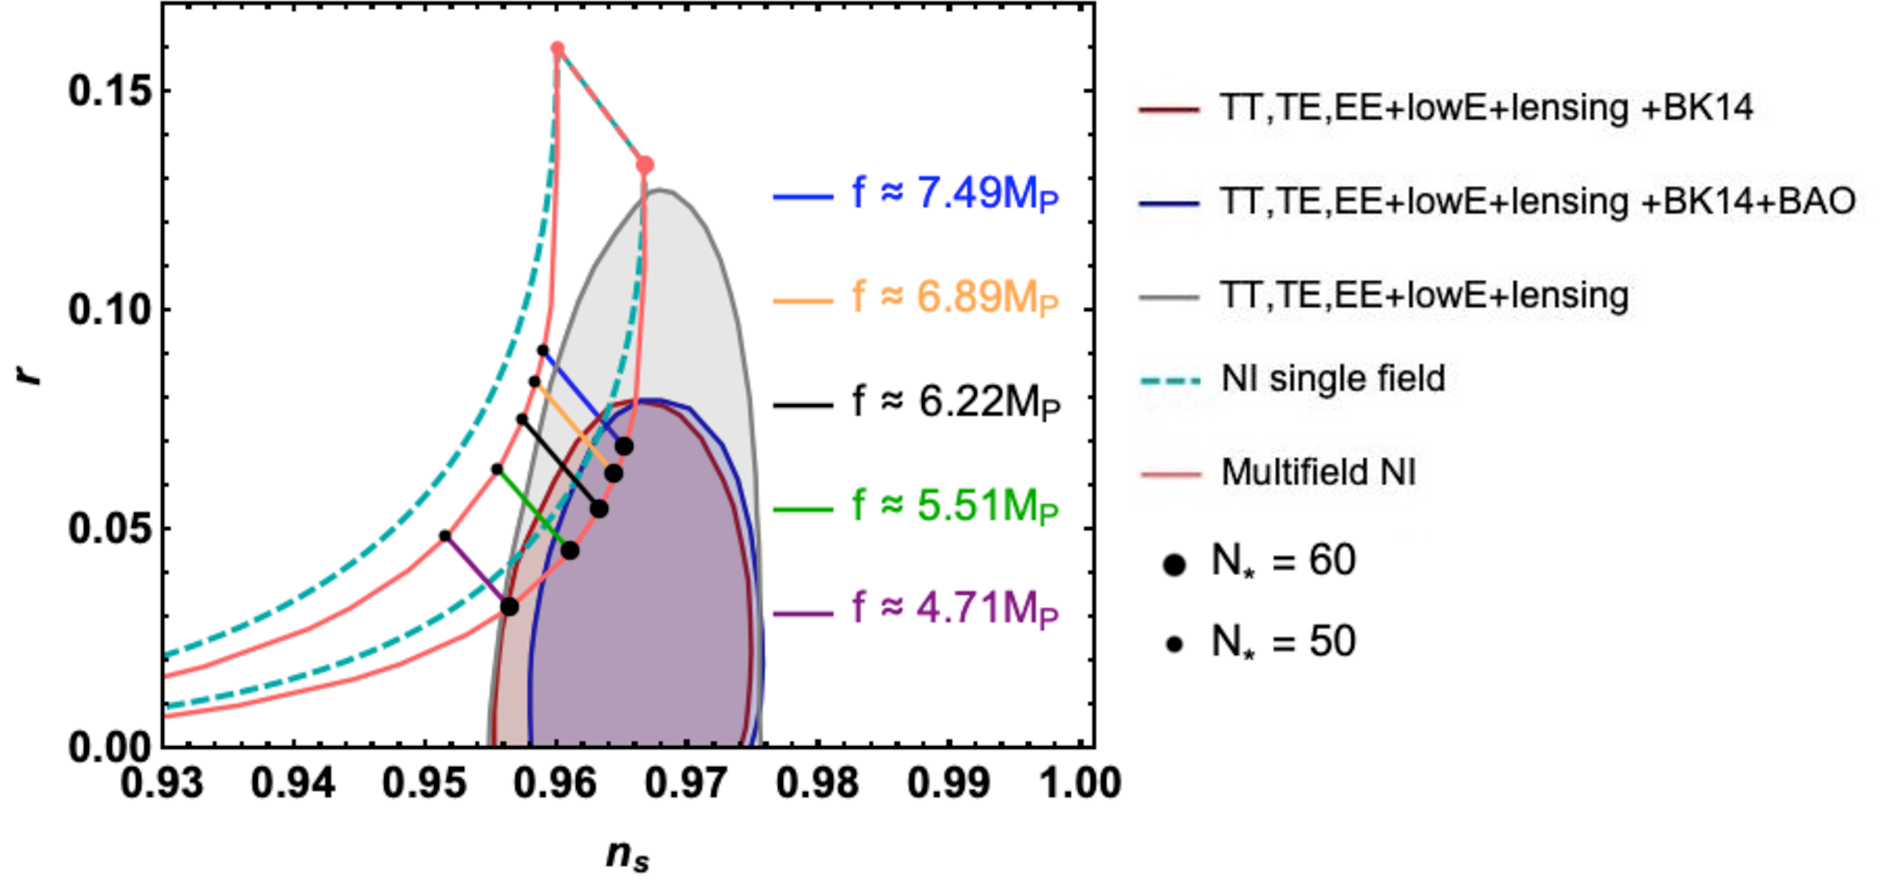
\includegraphics[width=.75\textwidth]{Sections/Figures/LT_nsr.pdf} 
\caption{ The $(n_s, r)$ plane for the strongly non-geodesic D5-brane multi-field  inflation model discussed in the text. $f$ is an  instantaneous  axion decay constant, which depends on the parameters of the model. The single-field natural inflation predictions are indicated by the cyan dashed curve,
while the fat D5-brane predictions follow the continuous curve. This figure is taken from \cite{Chakraborty:2019dfh}, which can be consulted for more details.} 
\label{fig:D5multi} 
\end{center}
\end{figure}

\subsubsection{Closed string multi-field inflation and spectator fields}

Thus far, we considered D-brane multi-field inflation models, focusing on the $(9-p)$ (open string) moduli associated to the positions of the brane as it moves in the internal space. In these models, the (reasonable) assumption is that all other (closed string) moduli have been stabilised via some of the mechanisms discussed in Sec. \ref{sec:MS}. Fields with other spins are also usually taken to be  unimportant during the inflationary evolution. We now review multi-field models of inflation in the closed string sector, as well as models with spectator fields of  spin 0 and/or 1. 

\subsubsection*{Alternative sources for curvature fluctuations  }

One of the characteristics of  inflationary scenarios involving more than one fluctuating scalar degree of freedom is the presence of entropy perturbations besides the adiabatic one. 

Multi-field models then offer alternative mechanisms to generate the density perturbations after the end of inflation. Two generic mechanisms for achieving such post-inflationary isocurvature-to-adiabatic conversion are  the  {\em curvaton}  \cite{Linde:1996gt,Lyth:2001nq,Moroi:2001ct} and the {\em modulated reheating} \cite{Dvali:2003em,Kofman:2003nx,Dvali:2003ar} scenarios. In the former case, the adiabatic curvature perturbation is generated from the decay of a spectator field, the curvaton, after the end of inflation and significant non-Gaussianity may be generated. 
In the modulated reheating scenario on the other hand, perturbations  in one or more  spectator fields modulate  the decay rate of the inflation field which gives rise to reheating.  This then  converts fluctuations of the spectator fields to density fluctuations in the post-inflationary universe. The observed curvature perturbations can again be non-Gaussian.  

In \cite{Burgess:2010bz} a string theory realisation of the curvaton  scenario  was proposed  where the inflaton is a  blow-up modulus (see blow-up inflation above) and a  fiber modulus plays the role of curvaton field.   This scenario 
 allows for large local non-Gaussianity at a level ${\mathcal O}(10)$, which is  in tension with the latest Planck constraints, $f_{\rm NL} =-0.9\pm 5.1$ (68\%C.L.) \cite{Planck:2019kim}.

Similarly, in \cite{Cicoli:2012cy} a string theory realisation of the modulated reheating scenario was presented,  where inflation is driven by a fibre modulus (see fibre inflation above), while a blow-up mode acts as a modulating field. Interestingly, in this scenario, local non-Gaussianity at a level  ${\mathcal O}({\rm few})$ can be produced generically, which is in agreement with the  latest Planck constraints on $f_{\rm NL}$. 

Finally, it was argued in \cite{Dimopoulos:2006ms,Dimopoulos:2011ws} that a vector field could play the role of the curvaton field. Moreover, the contribution of a vector field to the curvature perturbation will in general be statistically anisotropic, as shown in \cite{Dimopoulos:2008yv}. 
%
The possibility of realising the vector curvaton scenario in D3-brane models of inflation was investigated in \cite{Dimopoulos:2011pe}. The vector curvaton was identified with the $U(1)$ gauge field that lives on the world volume of a D3-brane, while the inflaton sector could arise from the same brane or some other sector. 
The dilaton was considered as a spectator field that modulates the evolution of the vector field. Given the current hints towards statistical anisotropies in the power spectrum and bispectrum \cite{Planck:2015igc}, the vector curvaton represents an interesting possibility.



\subsubsection*{Spectator Chromonatural Inflation (SCNI)}

We have discussed how string theory compactifications involve several spin-0 closed and open string moduli, which can have interesting implications for inflation. 
Spin-1 fields are also present and may generate  interesting phenomenology. Above, we discussed a spin-1 vector field as a candidate to generate the adiabatic perturbations, potentially leading to detectable statistical anisotropies. 

The Chern-Simons (CS) coupling between a rolling axion and a non-Abelian $SU(2)$ gauge field,  $\chi\,F_{\mu\nu}^a\tilde F^{a\,\mu\nu}$, where $F=dA-g\, A\wedge A$, with $g$ the gauge coupling, was introduced in \cite{Adshead:2012kp} to `slow down' the axion via its associated friction term.\footnote{See \cite{Maleknejad:2011sq,Maleknejad:2011jw,Adshead:2012qe,Sheikh-Jabbari:2012tom} for the  related scenario of gauge-flation and its relation to chromonatural inflation.} In this way, natural inflation could  proceed even  with a sub-Planckian decay constant, $f<\Mp$ (that is, in a steeper potential). This scenario is called chromonatural inflation (CNI). Interestingly, in this scenario, fluctuations in the gauge field source tensor and scalar modes. This is because the gauge field  
$A_\mu=A_\mu^aT_a$, (with $T^a$ the $SU(2)$ generators), can have a spatially isotropic configuration given by $A^a_i=Q(t)\delta_i^a$ at the background level, while its  fluctuations give rise to tensorial perturbations from $\delta A_j^a \sim B_{ij}\delta_i^a$, sourcing the equations of motion for the tensors at the linear level:  $\Box h_{ij} =-16\pi G \Pi_{ij}$, where $\Pi_{ij}$ is the tensor part of the energy momentum tensor fluctuations $\delta T_{\mu\nu}$. 
In particular, the tensor modes experience a transient growth in one of their polarisations,  $h_{\pm} = h_{\pm}^{\rm vacuum} + h_{\pm}^{\rm source}$, 
enhancing the amplitude of the gravitational waves and  leading to the production of a chiral tensor spectrum, distinguishable from the tensor spectrum that arises in vanilla inflation scenarios. Thanks to the extra source of primordial gravitational waves (PGW), these can be produced at observable levels even with sub-Planckian field excursions, thus evading the Lyth bound \eqref{eq:Lythbd}. 
Further investigation has shown, however, that in CNI it is not possible to simultaneously satisfy the bounds on $r$ and those on the scalar spectral index $n_s$ \cite{Adshead:2013qp,Adshead:2013nka}. An interesting proposal to alleviate this problem was proposed in \cite{Dimastrogiovanni:2016fuu}. The idea is to separate the inflationary sector from the gauge-axion sector, which  acts only as a spectator, thus called spectator chromonatural inflation (SCNI) in \cite{Holland:2020jdh}.
A common feature of CNI and SCNI is the need for a large
axion-gauge CS coupling, $\lambda$:
\be
\frac{\lambda }{4f} \,\chi\,F_{\mu\nu}^A\tilde F^{A\,\mu\nu}\,,
\ee
where $F=dA-g\, A\wedge A$, with $g$ the gauge coupling and both axion and gauge field canonically normalised. 
A successful SCNI, leading to a consistent background evolution and a large enhancement of the PGWs to observable levels without excessive backreaction of the
gauge field fluctuations, requires indeed   
($i$) $\frac{\lambda}{f}\Mp\gtrsim 10^4$, leading to typical values of $\lambda\gtrsim {\mathcal O}(10^2)$, sub-Planckian decay constants $f\lesssim  {\mathcal O}(10^{-1})$, and ($ii$) small gauge couplings $g\lesssim  {\mathcal O}(10^{-2})$. Obtaining these values represents a non-trivial theoretical challenge as pointed out  in \cite{Agrawal:2018mkd,Holland:2020jdh,Bagherian:2022mau}. 

Axions and non-Abelian gauge fields are common ingredients in string theory compactifications, and thus it is natural to ask whether the SCNI model can be realised successfully in a UV complete theory and, if not, what are the main challenges. Some attempts to do this have appeared in the literature recently. In \cite{DallAgata:2018ybl}, an embedding of  CNI in ${\cal N}=1$ supergravity was presented. 

Although, as we have mentioned, CNI is observationally
unviable, one could in principle add an inflationary sector into the setup in \cite{DallAgata:2018ybl}, keeping the axion-gauge sector as spectators, to construct a model of SCNI. However, the viability and phenomenology of such a model will need to be carefully analysed when adding more fields.

Later, in \cite{McDonough:2018xzh}, an embedding of SCNI into a  string theory scenario was presented. 
The  model considers  gaugino condensation on magnetised D7-branes in type IIB CY orientifold compactifications, and the axion associated to the 2-form potential $C_2$ present
in the compactification (used in \cite{Long:2014dta,Ben-Dayan:2014lca} to realise single-field natural inflation in string theory). The inflationary sector is given by a model of blow-up modulus inflation within the LVS. 
An explicit construction was not presented, and importantly, the  backreaction of the gauge field tensor fluctuations on the background was not considered. 

In view  of these results, \cite{Holland:2020jdh} considered in detail the requirements for a successful realisation of the SCNI scenario in explicit  string theory setups. Specifically, as already  mentioned, the construction should give ($i$) a successful background evolution, ($ii$) a sufficiently large enhancement of the tensor fluctuations to  detectable levels by future experiments, and ($iii$) a controllable backreaction from the gauge field tensor fluctuations.  The inflationary sector was given by blow-up inflation in the LVS framework,\footnote{Though a realisation with fibre inflation was also discussed in \cite{Holland:2020jdh}.} which, if taken alone as a single-field inflation, would give a tensor-to-scalar ratio that is too small to be observationally relevant.  Embedding into a multi-field K\"ahler inflation model requires 3 K\"ahler moduli and, in order to realise  SCNI, one needs to moreover introduce a spectator sector. This requires a fourth K\"ahler modulus and gaugino condensation on a multiply-wrapped magnetised stack of $N$ D7-branes, whose gauge field fluctuations couple to a $C_2$ axion. The full moduli stabilisation and cosmological evolution
of the inflaton, as well as the spectator sector, was analysed in detail and thus it possible to  explicitly identify the necessary parameters and their values in order to achieve the 3 goals stated above. Specifically, these parameters are: the magnetic flux $m$ on the D7-brane stack, the degree of the condensing group $N$, and the wrapping number $n$. The typical values for these parameters to achieve a successful SCNI are $(m,N,n) \sim {\cal O} (10^4,10^5,25)$. For the fibre inflation case, these numbers are slightly improved, $(m,N,n) \sim {\cal O} (10^2,10^3,1)$, though fibre inflation allows for a much larger tensor-to-scalar ratio. 



\subsubsection*{Multi-field Axion Monodromy}

Axion monodromy inflation represents an interesting scenario with a very rich phenomenology, in particular when considering multi-field extensions. Although there are no explicit string theory constructions of these, given their interesting phenomenology, we review here two  field theory models and a realisation in supergravity. 

\begin{enumerate}
\item[{\bf i.}] \underline{ Multiple axions Axion Monodromy}
Similar to N-flation, one possibility is to consider several axions whose  shift symmetry is broken at tree-level generating a leading power-law  term. This case was considered in \cite{Wenren:2014cga}, where it as shown that the spectral index is shifted red-wards from the single-field predictions. 

Later, in \cite{DAmico:2021vka,DAmico:2021fhz} the same generalisation was consider, with the distinctive feature that  inflation happens in two (or more) stages of monodromy inflation,  separated by non-inflating epochs, such as matter domination\footnote{Double inflation models have been considered in the past \cite{Silk:1986vc} to decouple
the spectrum on large and small scales. Models with multiple stages of inflation were called rollercoaster cosmology in \cite{DAmico:2020euu}.}. This model allows for a spectral index  which fits the CMB constraints, and $0.02 \lesssim r \lesssim 0.06$, which should be considered alongside the observational bound from BK-Planck 2020 $r\lesssim 0.3$   \cite{BICEP:2021xfz}. The authors also consider the possibility that the  first inflaton couples to a  $U(1)$ vector field,  producing  vectors near the end of the first stage of inflation, which in turn can source tensors during the intermediate matter epoch. These tensor modes turn out to be chiral and could be accessible to future gravitational wave experiments at different scales.


\item[{\bf ii.}] \underline{Axion-saxion Axion Monodromy}
While the models above focus on several axions, axions are usually coupled to their companion saxions, which are assumed to be stabilised in axionic inflation. 
However, the axion-saxion system can evolve cosmologically with very interesting effects. 
This was considered in \cite{Bhattacharya:2022fze}, which studied an ${\cal N}=1$ supergravity model with an axion-saxion system that evolves non-trivially, giving rise to several interesting effects: ($i$) the fields execute transient strong non-geodesic motion without the requirement of a large field space curvature\footnote{In \cite{Aragam:2021scu} it was shown that strong non-geodesic trajectories in supergravity seem to require large field space curvatures. }. This originates  from transient violations of slow-roll, $\eta\gtrsim1$, caused by the modulations  in the scalar potential. ($ii$) The non-trivial dynamics  lead to a large enhancement of the adiabatic power spectrum at small scales, providing the first concrete realisation of resonant features studied recently in the literature \cite{Fumagalli:2020nvq,Braglia:2020taf,Fumagalli:2021cel,Fumagalli:2021dtd}. These can lead to considerable production of light PBHs and a large and wide spectrum of induced GWs. The potential takes the simple form
\be\label{eq:VMAM}
\setlength\fboxsep{0.25cm}
\setlength\fboxrule{0.4pt}
\boxed{
V = \frac{M^2 }{\beta} \left(\rho^2 + \theta^2 + \frac{2\lambda}{M} \,e^{-b \rho} \left[\theta\,  \cos{(b \,\theta)}+  \rho\,  \sin{(b\, \theta)} + \frac{\lambda}{2M} \,e^{-b \rho}\right] \right)\,,}
\ee
where $\theta$ is the axion and $\rho$ the saxion, both of their  leading terms being quadratic\footnote{This potential arises from the following potentials: $\Mp^{-2}\,K = - \alpha \log[(\Phi + \bar \Phi)/\Mp -\beta S\bar S/\Mp^2]$ and
$W = S(M\Phi + i \lambda e^{- b\Phi} )$, where $S$ is a nilpotent superfield and $\Phi=\rho+ i \theta$ \cite{Ozsoy:2018flq,Bhattacharya:2022fze}.}. In Fig. \ref{fig:VMAM} we show the  
inflationary trajectory and in Fig.\ref{fig:psgw} we show the adiabatic   and GW spectra for a selection of parameters (see \cite{Bhattacharya:2022fze} for details). However, due to the large oscillations, the spectral index and tensor-to-scalar ratio at CMB scales have variations that violate current constraints. 

\begin{figure}[H]
\center{
\includegraphics[width=0.55\textwidth]{Sections/Figures/pot_3d_8050_try5.pdf}}
\caption{Inflationary trajectory of axion-saxion system as they move in the scalar potential \eqref{eq:VMAM} \cite{Bhattacharya:2022fze}.}
\label{fig:VMAM}
\end{figure}

\begin{figure}[H]
\center{
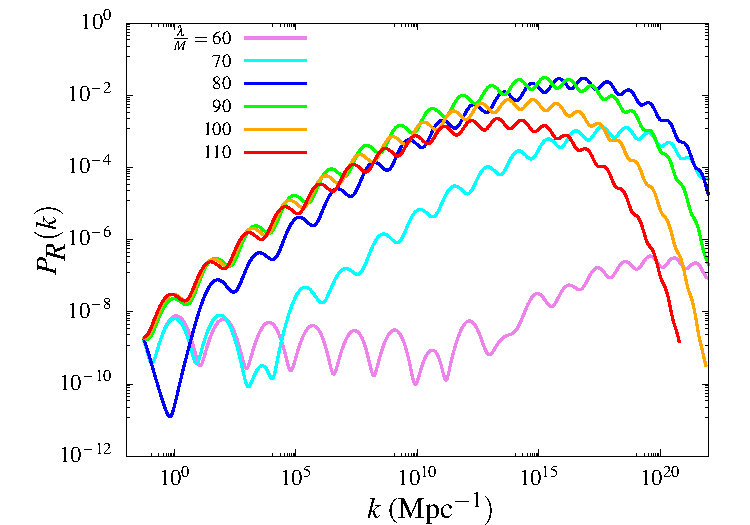
\includegraphics[width=0.49\textwidth]{Sections/Figures/ps_compare6.pdf}
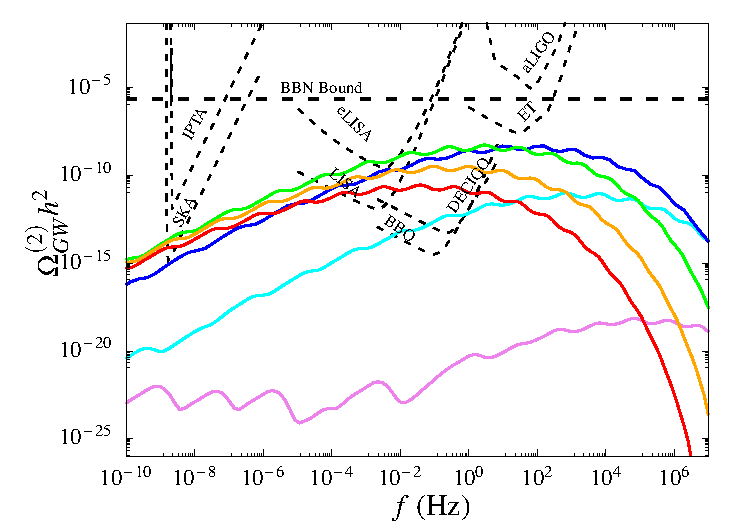
\includegraphics[width=0.48\textwidth]{Sections/Figures/GW_compare6.pdf}
}
\caption{Adiabatic (left) and GW (right)  spectra for a  selection  of parameters given in table 2 of \cite{Bhattacharya:2022fze}. The adiabatic power spectra are   computed using the code \texttt{PyTransport} \cite{Mulryne:2016mzv}. The left panel shows the variation of $P_{\mathcal{R}}(k)$ for different values of $\lambda /M$, with fixed $b=50$. The right panel shows the variation of $\Omega _{\rm GW}^{(2)}h^2$. 
}
\label{fig:psgw}
\end{figure}

\end{enumerate}

\enddocument

\newpage